%%%%%%%%%%%%%%%%%%%%%%%%%%%%%%%%%%%%%%%%%%%%%%%%%%%%%%%%%%%%
%%% LIVECOMS ARTICLE TEMPLATE
%%% ADAPTED FROM ELIFE ARTICLE TEMPLATE (8/10/2017)
%%%%%%%%%%%%%%%%%%%%%%%%%%%%%%%%%%%%%%%%%%%%%%%%%%%%%%%%%%%%
%%% PREAMBLE
\documentclass[9pt,bestpractices]{livecoms}
% Use the 'onehalfspacing' option for 1.5 line spacing
% Use the 'doublespacing' option for 2.0 line spacing
% use the 'lineno' option for adding line numbers.
% Please note that these options may affect formatting.

\usepackage{lipsum} % Required to insert dummy text
\usepackage[version=4]{mhchem}
\usepackage{siunitx}
\DeclareSIUnit\Molar{M}
\newcommand{\versionnumber}{1.6}  % you should update the minor version number in preprints and major version number of submissions.
\newcommand{\githubrepository}{\url{https://github.com/ejmaginn/TransportCheckList}}  %this should be the main github repository for this article
\graphicspath{{figures/}}
%%%%%%%%%%%%%%%%%%%%%%%%%%%%%%%%%%%%%%%%%%%%%%%%%%%%%%%%%%%%
%%% ARTICLE SETUP
%%%%%%%%%%%%%%%%%%%%%%%%%%%%%%%%%%%%%%%%%%%%%%%%%%%%%%%%%%%%
\title{Best Practices for Computing Transport Properties 1. Self-Diffusivity and Viscosity from Equilibrium Molecular Dynamics v\versionnumber}

%Edward Maginn (ejmaginn), Richard Elliott, Sunny Hwang, Daniel Roe (GitHub: drroe), Rich Messerly (ramess101)

\author[1*,\authfn{3}]{Edward J. Maginn}
\author[2*\authfn{6}]{Richard A. Messerly}
\author[3\authfn{7}]{Daniel J. Carlson}
\author[4\authfn{4}]{Daniel R. Roe}
\author[5\authfn{5}]{J. Richard Elliott}


\affil[1]{Department of Chemical and Biomolecular Engineering, The University of Notre Dame}
\affil[2]{Thermodynamics Research Center, National Institute of Standards and Technology}
\affil[3]{Chemical Engineering Department, Brigham Young University}
\affil[4]{Laboratory of Computational Biology, National Heart Lung and Blood Institute, National Institutes of Health}
\affil[5]{Department of Chemical and Biomolecular Engineering, The University of Akron}

\corr{ed@nd.edu}{EM}  % Correspondence emails.  Second {} are the appropriate authors initials.
\corr{daniel.roe@nih.gov}{DR}
\corr{elliot1@uakron.edu}{JRE}
\corr{richard.messerly@nist.gov}{RAM}
\corr{daniel.j.carlson@byu.edu}{DC}

%\contrib[\authfn{1}]{These authors contributed equally to this work}
%\contrib[\authfn{2}]{These authors also contributed to this work}

\blurb{This LiveCoMS document is maintained online on GitHub at \githubrepository; to provide feedback, suggestions, or help improve it, please visit the GitHub repository and participate via the issue tracker.\\
	\bigskip
	Contribution of the National Institute of Standards and Technology, not subject to US copyright.
}

%RAM: Still unclear why the bibliography is alphabetical. I tried updating the vancouver-livecoms.bst and livecoms.cls also.
\bibliographystyle{unsrt}

%\presentadd[\authfn{3}]{Maginn's Department, Institute, Country}
%\presentadd[\authfn{4}]{Roe's Department, Institute, Country}
%\presentadd[\authfn{5}]{Elliott's Department, Institute, Country}
%\presentadd[\authfn{6}]{Thermodynamics Research Center, National Institute of Standards and Technology, USA}
%\presentadd[\authfn{7}]{Chemical Engineering Department, Brigham Young University, USA}

%%%%%%%%%%%%%%%%%%%%%%%%%%%%%%%%%%%%%%%%%%%%%%%%%%%%%%%%%%%%
%%% ARTICLE START
%%%%%%%%%%%%%%%%%%%%%%%%%%%%%%%%%%%%%%%%%%%%%%%%%%%%%%%%%%%%

\begin{document}

\begin{frontmatter} %NOTE: to make the document single column, just take out the {frontmatter} sentinels
\maketitle

\begin{abstract}
%Please provide an abstract of no more than 250 words. Your abstract should explain the main contributions of your article, and should not contain any material that is not included in the main text.

The ability to predict transport properties (i.e. diffusivity, viscosity, conductivity) is one of the primary benefits of molecular simulation. Although most studies focus on the accuracy of the simulation output compared to experimental data, such a comparison primarily tests the adequacy of the force field (i.e. the model). By contrast, the reliability of different simulation methodologies for predicting transport properties is the focus of this manuscript. Unfortunately, obtaining reproducible estimates of transport properties from molecular simulation is not as straightforward as static properties. Therefore, this manuscript discusses the best practices that should be followed to ensure that the simulation output is reliable, i.e. is a valid representation of the force field implemented. We also discuss procedures to use so that the results are reproducible (i.e. can be obtained by other researchers following the same methods and procedures).

There are two classes by which transport properties are predicted: equilibrium molecular dynamics (EMD) and non-equilibrium molecular dynamics (NEMD). This manuscript presents the best practices for EMD, leaving NEMD for a future publication. As self-diffusivity and shear viscosity are the most prevalent transport properties found in the literature, the discussion will also be limited to these properties with the expectation that future publications will discuss best practices for thermal conductivity, ionic conductivity, and transport diffusivity.

\end{abstract}
\end{frontmatter}

%List of people to contact: Peter Cummings, Richard Rowley, Joachim Gross, Raj Khare, Richard Sadus, Ioannis Economou, Jadran Vrabec, Daniel Carlson, Chris Iocavella (any other Richards we can come up with)


%\section{Outline: Not included in publication}
%
%%This outline is not exactly what is being used currently
%General outline of equilibrium methods of self-diffusivity and viscosity for liquids:
%\begin{enumerate}
%	\item Introduction
%	\item Discussion of different methods within EMD (Green-Kubo, Einstein)
%	\item Summary of checklist for each property and method
%	\item General checklist items
%	\item Diffusion
%	\begin{enumerate}
%		\item Diffusion specific checklist items
%		\item Brief discussion of why we recommend Einstein over Green-Kubo?
%		\begin{enumerate}
%			\item Simulation setup that is specific to Einstein/diffusion
%		    \item Data analysis specific to Einstein/diffusion
%		    \item Common pitfalls for Einstein/diffusion
%		\end{enumerate}
%		\begin{enumerate}
%			\item Simulation setup that is specific to Green-Kubo/diffusion
%			\item Data analysis specific to Green-Kubo/diffusion
%			\item Common pitfalls for Green-Kubo/diffusion
%		\end{enumerate}
%	\end{enumerate}
%	\item Viscosity
%	\begin{enumerate}
%		\item Viscosity specific checklist items
%		\item Brief discussion of why we recommend Green-Kubo over Einstein?
%		\begin{enumerate}
%			\item Simulation setup that is specific to Green-Kubo/viscosity
%			\item Data analysis specific to Green-Kubo/viscosity
%			\item Common pitfalls for Green-Kubo/viscosity
%		\end{enumerate}
%        \begin{enumerate}
%        	\item Simulation setup that is specific to Einstein/viscosity
%        	\item Data analysis specific to Einstein/viscosity
%        	\item Common pitfalls for Einstein/viscosity
%        \end{enumerate}
%	\end{enumerate}
%\end{enumerate}


\section{Introduction}

Transport properties describe the rates at which mass, momentum, heat or charge move through a given substance. They involve mean squared displacements (MSDs) of molecules as the system evolves dynamically. In general, these properties can be computed by equilibrium molecular dynamics (EMD) or by non-equilibrium molecular dynamics (NEMD) methods. The EMD methods involve post-processing of a standard molecular dynamics (MD) trajectory while NEMD methods require modifications of the underlying equations of motion and/or boundary conditions of the system. Therefore, one advantage of EMD is that multiple transport properties can be obtained from a single simulation, whereas NEMD requires a separate simulation for each transport property of interest.

Some molecular simulation packages include built-in post-simulation analysis tools that automatically estimate transport properties from an EMD or NEMD simulation (e.g. Refs. \cite{LAMMPS,GROMACS,AMBER2018,NAMD,Brooks2009,ms2}). In addition, several stand-alone trajectory analysis tools are available which are intended to be simulation code agnostic (e.g. Refs. \cite{Roe2013,MDTraj,VMD}). However, there are often insufficient checks as to whether the actual underlying simulations are adequate for making these estimates. For this reason, we strongly discourage using these analysis tools as a ``black box,'' as no amount of post-processing can compensate for a poorly designed simulation. Following best practices for both the molecular simulation set-up and data analysis is imperative to ensure that meaningful predictions are obtained. The purpose of this document is to improve the quality of published results and to reduce the time required for a novice in the field to obtain meaningful and reliable results.

In addition to the present manuscript, we highly recommend reviewing this list of existing resources:
\begin{enumerate}
	\item Text books:
	\begin{enumerate}
		\item Ref. \cite{Allen2017}, pages 73--79, 274--281, and 292--296
		\item Ref. \cite{Frenkel2002}, pages 87--90 and 509--523
		\item Ref. \cite{Leach2001}, pages 374--382
	\end{enumerate}
	\item Class notes
	\begin{enumerate}
		\item Ref. \cite{PanaNotes}
		\item Ref. \cite{KofkeNotes}
		\item Ref. \cite{MaginnNotes}
		\item Ref. \cite{ShellNotes}

	\end{enumerate}
	\item Published articles
	\begin{enumerate}
		\item Ref. \cite{Chen2009}
		\item Ref. \cite{Hess2002}
		\item Ref. \cite{Nieto2015}, pages 13139--13140
		\item Ref. \cite{Ungerer2007}
	\end{enumerate}
	\item Software manuals
	\begin{enumerate}
		\item Ref. \cite{LAMMPS}
		\item Ref. \cite{GROMACS}
		\item Ref. \cite{AMBER2018}
	\end{enumerate}
\end{enumerate}
Most text books and class notes provide a thorough discussion of EMD/NEMD theory with little discussion of practical considerations. Review articles tend to focus on the numerical advantages and disadvantages of different methods but assume that the reader already understands the subtleties of implementing each method. Furthermore, although software manuals describe some of the theory and implementation of these methods in their respective environments, the documentation is typically insufficient for someone not familiar with best practices for estimating transport properties. This document supplements the existing literature by providing a succinct checklist and discussing common pitfalls. We also provide some suggestions and recommendations based on our own experience, but ultimately it is up to the individual researcher to test and validate their methods.

\section{Equilibrium Molecular Dynamics (EMD) for Estimating Transport Properties}

It is most convenient to consider compiling the transport properties as an implicit part of any equilibrium MD simulation. The added computational overhead is relatively small, especially for the self-diffusivity. The main caveat is that longer simulations than normal may be required to achieve reasonable averages.

The general formula for computing a transport property via an EMD simulation is given as

\begin{equation} \label{eq:Green-Kubo}
\gamma = \int_{0}^{\infty}dt\langle\dot{\xi}(t)\dot{\xi}(0)\rangle
\end{equation}
where $\gamma$ is the transport coefficient (within a multiplicative constant), $\xi$ is the perturbation in the Hamiltonian associated with the particular transport property under consideration and $\dot{\xi}$ signifies a time derivative. Integrals of the form given by Equation \ref{eq:Green-Kubo} are known as “Green-Kubo” integrals. It is easy to show that an integrated form of Equation \ref{eq:Green-Kubo} results in an equivalent expression for $\gamma$ known as the “Einstein” formula

\begin{equation} \label{eq:Einstein}
\gamma = \lim_{t\to\infty} \frac{\langle (\xi(t)-\xi(0))^2 \rangle}{2t} = \frac{1}{2} \lim_{t\to\infty} \frac{d}{dt} \langle (\xi(t)-\xi(0))^2 \rangle
\end{equation}
where the derivative form is often preferred.

For self-diffusivity, $\xi$ is the Cartesian atom position $(r_{\alpha})$ and the time correlation function, $\dot{\xi}$, in Equation \ref{eq:Green-Kubo} is of the molecular velocities $(v_{\alpha})$. For the shear viscosity, the integral in Equation \ref{eq:Green-Kubo} is of the time correlation of the off-diagonal elements of the stress tensor. For the thermal conductivity the integral is over the energy current, and for the ionic conductivity the integral is over the ionic current. Table \ref{tab:EMD_equations} provides the relevant equations for self-diffusivity $(D)$ and shear viscosity $(\eta)$, as these properties are the focus of this work.

% The relevant equations for self-diffusivity and shear viscosity are provided in Table \ref{tab:EMD_equations}.

% I think this table could be useful -ramess101

%\begin{table}[bt]
%	\caption{\label{tab:EMD_equations}Equilibrium molecular dynamics equations.}
%	% Use ``S'' column identifier to align on decimal point
%	% ``l'' left aligns text in the column
%	% ``r'' right aligns text in the column
%	% ``c'' right aligns text in the column
%	% & separates columns, \\ ends the row.
%
%	\begin{tabular}{l l l l l}
%		\toprule
%		Property & $\gamma$          & $\xi$                        & Equation \ref{eq:Green-Kubo}    & Equation \ref{eq:Einstein}     \\
%		\midrule
%		Self-diffusion     & $D$ & $x$          & $\int_{0}^{\infty}dt\langle v_{x,i}(t) v_{x,i}(0)\rangle$    & $\frac{1}{2t}\langle (x_i(t)-x_i(0))^2 \rangle$   \\
%		Shear viscosity     & $\eta$       & $x v_y$           & $\beta V \int_{0}^{\infty}dt\langle P_{x,y}(t) P_{x,y}(0)\rangle$    & $\frac{m^2\beta}{2t}\langle (x_i(t)v_{y,i}(t)-x_i(0)v_{y,i}(0))^2 \rangle$  \\
%		Thermal conductivity      & $\lambda$      & $x E$              & $ \frac{k\beta^2}{V} \int_{0}^{\infty}dt\langle S_{x}(t) S_{x}(0)\rangle$    & $\frac{k\beta^2}{2Vt}\langle \left(x_i(t)(E_i(t)-\langle E \rangle)-x_i(0)(E_i(0)-\langle E \rangle)\right)^2 \rangle$  \\
%		\bottomrule
%	\end{tabular}
%$P_{x,y}(t) = \frac{1}{V} \sum_{i=1}^{N} \left( \frac{p_{x,i}(t)p_{y,i}(t)}{m} + x_i(t) f_{y,i}(t) \right)$
%\newline
%$S_{x}(t) = \frac{d}{dt} \sum_{i=1}^{N} \left( x_i(t) (E_i(t) - \langle E \rangle) \right)$.
%\end{table}

% Since this paper focuses on diffusion and viscosity I have removed conductivity. I also modified the equations somewhat. -RAM
%\begin{table}[bt]
%	\caption{\label{tab:EMD_equations}Equilibrium molecular dynamics equations.}
%	% Use ``S'' column identifier to align on decimal point
%	% ``l'' left aligns text in the column
%	% ``r'' right aligns text in the column
%	% ``c'' right aligns text in the column
%	% & separates columns, \\ ends the row.
%
%	\begin{tabular}{l l l l l}
%		\toprule
%		Property & $\gamma$          & $\xi$                        & Equation \ref{eq:Green-Kubo}    & Equation \ref{eq:Einstein}     \\
%		\midrule
%		Self-diffusion     & $D$ & $\alpha$          & $\int_{0}^{\infty}dt\langle v_{\alpha,i}(t) v_{\alpha,i}(0)\rangle$    & $\frac{1}{2t}\langle (\alpha_i(t)-\alpha_i(0))^2 \rangle$   \\
%		Shear viscosity     & $\eta$       & $\alpha \dot{\beta}$           & $\frac{V}{k_bT} \int_{0}^{\infty}dt\langle P_{\alpha,\beta}(t) P_{\alpha,\beta}(0)\rangle$    & $\frac{m^2}{2k_bTVt}\langle (\alpha_i(t)\dot{\beta_i}(t)-\alpha_i(0)\dot{\beta_i}(0))^2 \rangle$  \\
%		\bottomrule
%	\end{tabular}
%\newline
%$P_{\alpha,\beta}(t) = \frac{1}{V} \sum_{i=1}^{N} \left( \frac{p_{\alpha,i}(t)p_{\beta,i}(t)}{m} + \alpha_i(t) \ddot{\beta_i}(t) \right)$
%\newline
%$\alpha$, $\beta = x, y, $ or $z$ coordinates
%\end{table}

\begin{table*}[tb]
	\caption{\label{tab:EMD_equations}Equilibrium molecular dynamics equations.}
	% Use ``S'' column identifier to align on decimal point
	% ``l'' left aligns text in the column
	% ``r'' right aligns text in the column
	% ``c'' right aligns text in the column
	% & separates columns, \\ ends the row.

	\begin{tabular}{l l l l l}
		\toprule
		Property & $\gamma$          & $\xi$                        & Green-Kubo (Equation \ref{eq:Green-Kubo})    & Einstein (Equation \ref{eq:Einstein})     \\
		\midrule
		Self-diffusivity     & $D$ & $r_{\alpha}$          & $ \displaystyle \frac{1}{\rm d} \int_{0}^{\infty}dt\left\langle \frac{1}{N} \sum_{i=1}^{N} v_{\alpha,i}(t) v_{\alpha,i}(0)\right\rangle_{t_0}$    & $ \displaystyle \frac{1}{\rm 2d} \lim_{t\to\infty} \frac{d}{dt} \left\langle \frac{1}{N} \sum_{i=1}^{N} |r_{\alpha,i}(t)-r_{\alpha,i}(0)|^2 \right\rangle_{t_0}$   \\
		Shear viscosity     & $\eta$       & $r_\alpha v_\beta$           & $ \displaystyle \frac{V}{k_bT} \int_{0}^{\infty}dt\left\langle \tau_{\alpha,\beta}(t) \tau_{\alpha,\beta}(0)\right\rangle_{t_0}$    & $ \displaystyle \frac{V}{2k_bT} \lim_{t\to\infty} \frac{d}{dt} \left\langle \left(\int_{0}^{t}dt' \tau_{\alpha,\beta}(t')\right)^2 \right\rangle_{t_0}$  \\
		\bottomrule
	\end{tabular}
	\newline
	%$P_{\alpha,\beta}(t) = \frac{1}{V} \sum_{i=1}^{N} \left( \frac{p_{\alpha,i}(t)p_{\beta,i}(t)}{m} + \alpha_i(t) \ddot{\beta_i}(t) \right)$
	$\alpha$, $\beta = x, y, $ or $z$ Cartesian coordinates of the atoms or molecule center of mass \newline
	$\rm d =$ dimensionality (1,2, or 3) \newline
	$N=$ number of atoms or molecules (see Sec.\ \ref{sec:General: Clear communication}) \newline
%	$V=$ volume \newline
	$k_b=$ Boltzmann constant \newline
	$\tau_{\alpha,\beta}(t) = \frac{1}{V} \sum_{i=1}^{N} \left( m v_{\alpha,i}(t) v_{\beta,i}(t) + r_{\alpha,i}(t) f_{\beta,i}(t) \right) , \alpha \ne \beta$ \newline
	$f_{\beta,i}$ is the force acting on particle $i$ in direction $\beta$ \newline
	$\langle \cdots \rangle_{t_0}$ denotes an average over time origins (see Sec.\ \ref{sec:General: Improve precision})
\end{table*}

Although both Equation \ref{eq:Green-Kubo} (Green-Kubo) and Equation \ref{eq:Einstein} (Einstein) are theoretically rigorous, in practice one method is often preferred depending on the property being estimated. In the case of self-diffusivity, we recommend the Einstein (MSD) approach. In contrast, for shear viscosity we typically recommend Green-Kubo, although for some systems the Einstein approach may be preferable. As the simulation set-up and computational cost are essentially the same for the Green-Kubo and Einstein approaches, the primary difference is the post-simulation data analysis required. Precision and reproducibility of the estimated value are key factors for selecting between the Green-Kubo or Einstein methods. For this reason, we emphasize the importance of proper and clearly communicated data analysis and rigorous uncertainty quantification.

\section{Checklist} \label{Checklist}

This section provides an overview of the checklist items for each property $(D$ and $\eta)$ and method (Green-Kubo and Einstein). Detailed discussions for each checklist item are found in Sections \ref{sec:General}-\ref{sec:Viscosity}.

%I envision this being a table that has links to the different sections for each property
%\begin{enumerate}
%	\item Simulation set-up
%	\begin{enumerate}
%		\item Correct ensemble
%		\item Sufficient samples
%		\begin{enumerate}
%			\item Number of replicates
%			\item Simulation length
%			\item Output frequency
%		\end{enumerate}
%	    \item System size
%	\end{enumerate}
%    \item Post-simulation analysis
%    \begin{enumerate}
%    	\item Tricks to improve precision
%    	\item Clear communication of how $D$ or $\eta$ is obtained from Equation \ref{eq:Green-Kubo} or \ref{eq:Einstein}
%    	\item Uncertainty in $D$ or $\eta$ not attributed to force field deficiencies
%    \end{enumerate}
%    \item Common pitfalls
%    \item Special considerations
%\end{enumerate}

\begin{Checklists*}[p!]
	\begin{checklist}{Checklist for Computing Self-Diffusivity with Einstein Equilibrium Approach}
		\begin{itemize}
			\item
			\textbf{Simulation set-up.} No amount of data analysis can compensate for a poorly designed experiment. It is imperative that the simulation sufficiently samples the relevant region of phase space.
			\begin{itemize}
				\item Sample from the correct ensemble. See Sec.\ \ref{sec:General: Correct Ensemble}.
				\item Increase the information extracted from simulation results.
				\begin{itemize}
					\item Perform multiple replicate simulations. See Sec.\ \ref{sec:General: Replicate simulations}.
					\item Ensure that simulations are sufficiently long. See Sec.\ \ref{sec:Self-Diffusivity:Einstein: Simulation length}.
					\item Increase the output frequency. See Sec.\ \ref{sec:Self-Diffusivity:Einstein: Output frequency}.
				\end{itemize}
				\item Check for system size effects. See Sec.\ \ref{sec:Self-Diffusivity:General: Finite size}
			\end{itemize}
			\vspace{-0.325\baselineskip} %Line spacing after a sub-list is too large

			\item
			\textbf{Post-simulation data analysis.} Data analysis is key for obtaining reproducible and meaningful estimates of $D$.
			\begin{itemize}
				\item Improve precision by averaging over:
				\begin{itemize}
					\item Multiple time origins. See Sec.\ \ref{sec:General: Improve precision}.
					\item $N$ molecules. See Sec.\ \ref{sec:General: Improve precision}.
					\item Three dimensions (xx, yy, zz). See Sec.\ \ref{sec:General: Improve precision}.
					\item Multiple replicate simulations. See Sec.\ \ref{sec:General: Replicate simulations}.
				\end{itemize}
				\item Clearly communicate how $D$ is obtained from Equation \ref{eq:Einstein}. See Secs.\ \ref{sec:General: Clear communication}, \ref{sec:Self-Diffusivity:General: Data analysis}, and \ref{sec:Self-Diffusivity:Einstein: Data analysis}.
				\item Report the uncertainty in $D$:
				\begin{itemize}
					\item Bootstrap replicate simulations. See Sec.\ \ref{sec:General: Uncertainty}.
					\item Perform sensitivity analysis, i.e. variation in $D$ with respect to the time cut-off, etc. See Sec.\ \ref{sec:Self-Diffusivity:Einstein: Data analysis}.
				\end{itemize}
			\end{itemize}
		    \vspace{-0.325\baselineskip} %Line spacing after a sub-list is too large

			\item
			\textbf{Common pitfalls.} Double-check that your results are not plagued by one of the common pitfalls. See Sec.\ \ref{sec:General: Common pitfalls}.
			
			\item
			\textbf{Validation.} Compare your results with those from a reputable source. See Sec.\ \ref{sec:General: Validation}.

			\item
			\textbf{Special topics.} Check if your system of interest requires some special considerations. See Sec.\ \ref{sec:Self-Diffusivity Special topics}.

		\end{itemize}
	\end{checklist}
\end{Checklists*}

\begin{Checklists*}[p!]
	\begin{checklist}{Checklist for Computing Viscosity with Green-Kubo Equilibrium Approach}
		\begin{itemize}
			\item
			\textbf{Simulation set-up.} No amount of data analysis can compensate for a poorly designed experiment. It is imperative that the simulation sufficiently samples the relevant region of phase space.
			\begin{itemize}
				\item Sample from the correct ensemble. See Sec.\ \ref{sec:General: Correct Ensemble}.
				\item Increase the information extracted from simulation results.
				\begin{itemize}
					\item Perform multiple replicate simulations. See Sec.\ \ref{sec:General: Replicate simulations}.
					\item Ensure that simulations are sufficiently long. See Sec.\ \ref{sec:Viscosity:General: Simulation length}.
					\item Increase the output frequency. See Sec.\ \ref{sec:Viscosity:General: Output frequency}.
				\end{itemize}
				\item Check for system size effects. See Sec.\ \ref{sec:Viscosity:General: Finite size}.
			\end{itemize}
			\vspace{-0.325\baselineskip} %Line spacing after a sub-list is too large
			
			\item
			\textbf{Post-simulation data analysis.} Data analysis is key for obtaining reproducible and meaningful estimates of $\eta$.
			\begin{itemize}
				\item Improve precision by averaging over multiple:
				\begin{itemize}
					\item Time origins. See Sec.\ \ref{sec:General: Improve precision}.
					\item Stress tensor elements (three off-diagonal or all six). See Sec.\ \ref{sec:Viscosity:General: Improved precision}.
					\item Replicate simulations. See Sec.\ \ref{sec:General: Replicate simulations} and \ref{sec:Viscosity:General: Improved precision}.
				\end{itemize}
				\item Clearly communicate how $\eta$ is obtained from Equation \ref{eq:Green-Kubo}. See Secs.\ \ref{sec:General: Clear communication} and \ref{sec:Viscosity:Green-Kubo: Data analysis}.
				\item Report the uncertainty in $\eta$:
				\begin{itemize}
					\item Bootstrap replicate simulations. See Sec.\ \ref{sec:General: Uncertainty}.
					\item Perform sensitivity analysis, i.e. variation in $\eta$ with respect to the time cut-off, fitting model, etc. See Sec.\ \ref{sec:Viscosity:Green-Kubo: Data analysis}.
				\end{itemize}
			\end{itemize}
			\vspace{-0.325\baselineskip} %Line spacing after a sub-list is too large
			
			\item
			\textbf{Common pitfalls.} Double-check that your results are not plagued by one of the common pitfalls. See Sec.\ \ref{sec:General: Common pitfalls}.
			
			\item
			\textbf{Validation.} Compare your results with those from a reputable source. See Sec.\ \ref{sec:General: Validation}.
			
			\item
			\textbf{Special topics.} Check if your system of interest requires some special considerations. See Sec.\ \ref{sec:Viscosity Special topics}.
			
		\end{itemize}
	\end{checklist}
\end{Checklists*}

\begin{Checklists*}[p!]
	\begin{checklist}{Checklist for Computing Self-Diffusivity with Green-Kubo Equilibrium Approach}
		\begin{itemize}
			\item
			\textbf{Simulation set-up.} No amount of data analysis can compensate for a poorly designed experiment. It is imperative that the simulation sufficiently samples the relevant region of phase space.
			\begin{itemize}
				\item Sample from the correct ensemble. See Sec.\ \ref{sec:General: Correct Ensemble}.
				\item Increase the information extracted from simulation results.
				\begin{itemize}
					\item Perform multiple replicate simulations. See Sec.\ \ref{sec:General: Replicate simulations}.
					\item Ensure that simulations are sufficiently long. See Sec.\ \ref{sec:Self-Diffusivity:Green-Kubo: Simulation length}
					\item Increase the output frequency. See Sec.\ \ref{sec:Self-Diffusivity:Green-Kubo: Output frequency}.
				\end{itemize}
				\item Check for system size effects. See Sec.\ \ref{sec:Self-Diffusivity:General: Finite size}.
			\end{itemize}
			\vspace{-0.325\baselineskip} %Line spacing after a sub-list is too large

			\item
			\textbf{Post-simulation data analysis.} Data analysis is key for obtaining reproducible and meaningful estimates of $D$.
			\begin{itemize}
				\item Improve precision by averaging over:
				\begin{itemize}
					\item Multiple time origins. See Sec.\ \ref{sec:General: Improve precision}.
					\item $N$ molecules. See Sec.\ \ref{sec:General: Improve precision}.
					\item Three dimensions (xx, yy, zz). See Sec.\ \ref{sec:General: Improve precision}.
					\item Multiple replicate simulations. See Sec.\ \ref{sec:General: Replicate simulations}.
				\end{itemize}
				\item Clearly communicate how $D$ is obtained from Equation \ref{eq:Green-Kubo}. See Secs.\ \ref{sec:General: Clear communication}, \ref{sec:Self-Diffusivity:General: Data analysis}, and \ref{sec:Self-Diffusivity:Green-Kubo: Data analysis}.
				\item Report the uncertainty in $D$:
				\begin{itemize}
					\item Bootstrap replicate simulations. See Sec.\ \ref{sec:General: Uncertainty}.
					\item Perform sensitivity analysis, i.e. variation in $D$ with respect to the time cut-off, etc. See Sec.\ \ref{sec:Self-Diffusivity:Green-Kubo: Data analysis}.
				\end{itemize}
			\end{itemize}
			\vspace{-0.325\baselineskip} %Line spacing after a sub-list is too large

			\item
			\textbf{Common pitfalls.} Double-check that your results are not plagued by one of the common pitfalls. See Sec.\ \ref{sec:General: Common pitfalls}.

			\item
			\textbf{Validation.} Compare your results with those from a reputable source. See Sec.\ \ref{sec:General: Validation}.

			\item
			\textbf{Special topics.} Check if your system of interest requires unique considerations. See Sec.\ \ref{sec:Self-Diffusivity Special topics}.

		\end{itemize}
	\end{checklist}
\end{Checklists*}

\begin{Checklists*}[p!]
	\begin{checklist}{Checklist for Computing Viscosity with Einstein Equilibrium Approach}
		\begin{itemize}
			\item
			\textbf{Simulation set-up.} No amount of data analysis can compensate for a poorly designed experiment. It is imperative that the simulation sufficiently samples the relevant region of phase space.
			\begin{itemize}
				\item Sample from the correct ensemble. See Sec.\ \ref{sec:General: Correct Ensemble}.
				\item Increase the information extracted from simulation results.
				\begin{itemize}
					\item Perform multiple replicate simulations. See Sec.\ \ref{sec:General: Replicate simulations}.
					\item Ensure that simulations are sufficiently long. See Sec.\ \ref{sec:Viscosity:General: Simulation length}.
					\item Increase the output frequency. See Sec.\ \ref{sec:Viscosity:General: Output frequency}.
				\end{itemize}
				\item Check for system size effects. See Sec.\ \ref{sec:Viscosity:General: Finite size}.
			\end{itemize}
			\vspace{-0.325\baselineskip} %Line spacing after a sub-list is too large

			\item
			\textbf{Post-simulation data analysis.} Data analysis is key for obtaining reproducible and meaningful estimates of $\eta$.
			\begin{itemize}
				\item Improve precision by averaging over multiple:
				\begin{itemize}
					\item Time origins. See Sec.\ \ref{sec:General: Improve precision}.
					\item Stress tensor elements (three off-diagonal or all six). See Sec.\ \ref{sec:Viscosity:General: Improved precision}.
					\item Replicate simulations. See Sec.\ \ref{sec:General: Replicate simulations} and \ref{sec:Viscosity:General: Improved precision}.
				\end{itemize}
				\item Clearly communicate how $\eta$ is obtained from Equation \ref{eq:Einstein}. See Secs.\ \ref{sec:General: Clear communication} and \ref{sec:Viscosity:Einstein: Data analysis}.
				\item Report the uncertainty in $\eta$:
				\begin{itemize}
					\item Bootstrap replicate simulations. See Sec.\ \ref{sec:General: Uncertainty}.
					\item Perform sensitivity analysis, i.e. variation in $\eta$ with respect to the time cut-off, fitting model, etc. See Sec.\ \ref{sec:Viscosity:Einstein: Data analysis}.
				\end{itemize}
			\end{itemize}
			\vspace{-0.325\baselineskip} %Line spacing after a sub-list is too large

			\item
			\textbf{Common pitfalls.} Double-check that your results are not plagued by one of the common pitfalls. See Sec.\ \ref{sec:General: Common pitfalls}.

			\item
			\textbf{Validation.} Compare your results with those from a reputable source. See Sec.\ \ref{sec:General: Validation}.

			\item
			\textbf{Special topics.} Check if your system of interest requires some special considerations. See Sec.\ \ref{sec:Viscosity Special topics}.

		\end{itemize}
	\end{checklist}
\end{Checklists*}

\section{General transport checklist items} \label{sec:General}

\subsection{General transport: Simulation set-up} \label{sec:General Simulation Setup}

\subsubsection{Correct Ensemble} \label{sec:General: Correct Ensemble}

For a liquid solution, it is safest to run in the microcanonical ($NVE$, constant number of molecules, volume, energy) ensemble. This is because thermostats required to maintain constant temperature and barostats required to maintain constant pressure can interfere with the dynamics of the system, and thus the resulting transport properties can be skewed. However, it is most common to desire $D$ and $\eta$ at a specified temperature $(T)$ and pressure $(P)$. This requires performing a series of simulations in different ensembles:
\begin{enumerate}
	\item $NPT$ ensemble at desired $T$ and $P$ until the system density has properly equilibrated
	\item $NVT$ ensemble where the volume is set such that the density is the average density computed from the $NPT$ run
	\item $NVE$ ensemble where the final configuration of the $NVT$ run is used as the initial configuration
\end{enumerate}
% Do we really just want the last configuration? Should we randomly select a configuration from production? Or a few configurations to run in parallel? Or somehow find an "average" configuration? My concern is just, what if the last configuration happens to be a higher energy sample (or lower probability if coming at it from a Monte Carlo point of view)? -ramess101
It is important that each step consist of both an equilibration and production period. The average pressure and temperature for the $NVE$ production run are computed and should be close to (but not exactly the same) as the input $P$ and $T$ to the original $NPT$ run. These average pressures and temperatures must be reported along with the self-diffusivity and/or viscosity.

%The user should generate multiple starting states that can be used to determine error estimation (see item \ref{item:uncertainty}).

Note that, although the best practice is to use the $NVE$ ensemble (Steps 1 to 3), it is common to see values reported using the $NPT$ (just Step 1) or $NVT$ (Steps 1 and 2) ensemble. We strongly discourage the use of the $NPT$ ensemble alone, because barostats (which alter positions through volume changes) greatly affect the dynamics of a system. In contrast, the $NVT$ ensemble has been implemented successfully for transport property calculations and is quite common, especially for viscosity. For example, Fanourgakis et al. reported that the $NVT$ and $NVE$ ensembles provide nearly identical results for viscosity \cite{Fanourgakis2012}. A study by Basconi and Shirts \cite{Shirts2013} reached a similar conclusion, and provides guidelines for how thermostats should be applied when computing transport properties. To summarize their results, $NVT$ simulations with velocity-scaling thermostats (e.g. Berendsen \cite{Berendsen1984}, stochastic rescaling \cite{Bussi2007}, and Nos{\'e}-Hoover \cite{Nose1984} thermostats) and a wide range of coupling strengths (0.1, 1, and 10 ps) provide $D$ and $\eta$ values that are statistically indistinguishable from the $NVE$ ensemble estimates. By contrast, velocity-randomizing algorithms (e.g. Andersen thermostat \cite{Andersen1980} and Langevin dynamics \cite{Hess2008}) with strong coupling (0.1 and 1 ps) dramatically decrease $D$ and increase $\eta$ relative to the $NVE$ ensemble values. Therefore, we recommend using either the $NVT$ or $NVE$ ensemble, with $NVE$ being preferred. If $NVT$ simulations are used, we recommend judiciously selecting the thermostat and coupling strength by consulting Refs. \cite{Fanourgakis2012,Shirts2013}.

%Furthermore, although most studies use the average density in Step 2, it is important to consider the uncertainty in $D$ or $\eta$ that arises from the uncertainty in $\rho$. Although it is not common to account for this source of uncertainty, we recommend %RAM: This issue is not as important as long as you report the uncertainty in P and/or T in your final simulation.

 %Although this may be the best practice, it appears to me that a large number of practitioners run their production simulations in the $NPT$ ensemble. Should we point this out? I.e. should we say something like "although it is common to see values reported from the $NPT$ ensemble..."? That way the reader will know why our recommendation seems to differ from what they find in the literature. -ramess101
% What about for the gas phase? -RAM

\subsubsection{Replicate simulations} \label{sec:General: Replicate simulations}

To smooth noise in the Green-Kubo integral or Einstein slope, we recommend generating independent replicate trajectories (i.e. different initial configurations or random seed to initialize velocities). The primary advantage of performing replicates as opposed to one longer simulation is the computational speed-up. Figure 2 in Ref. \cite{Payal2012} demonstrates that an average of 10 short replicate simulations converges to the same value as a single long simulation. Since these replicates can be performed in parallel, the time required to obtain the result is reduced, although the CPU time may be the same or more.

%\begin{figure}[htb!]
%	\centering
%	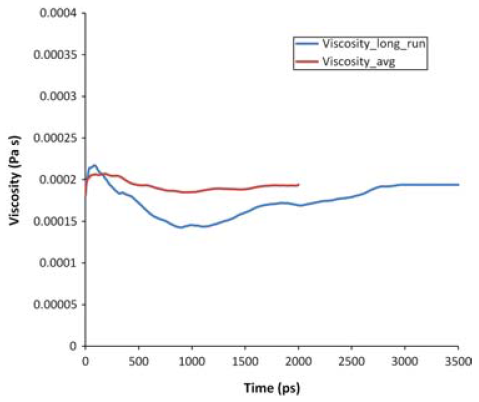
\includegraphics[width=3.2in]{PayalFig2.png}
%	\caption{Green-Kubo viscosity plot. Copied from Figure 2 of Ref.\ \cite{Payal2012}. Red curve represents the average viscosity over 10 independent 2 ns trajectories whereas the blue curve is obtained from a single 4 ns simulation. For further details, see Ref. \cite{Payal2012}. {\bf Note: When I went to Taylor and Francis to request re-use of this figure, they asked for 315 dollars. I think we need a substitute.}}
%	\label{fig:PayalFig2}
%\end{figure}

The uncertainty is inversely proportional to the square root of the number of replicates (see Figure 7 of Ref. \cite{Zhang2015} and Figure 8 of Ref. \cite{Ma2017}), so increasing the number of replicates is a simple, fast, and direct way to reduce the uncertainty. For example, the fluctuations in $\eta$ are much smaller for the average of 10 replicates compared to that of a single longer simulation (see Figure 2 of Ref. \cite{Payal2012}). As fluctuations in $\eta$ are typically much larger than $D$, more replicate simulations are required for estimating viscosity (see Sec.\ \ref{sec:Viscosity:General: Improved precision}).

In addition, replicate simulations are useful if a single simulation does not adequately sample phase space, i.e. is trapped in a local minimum or has slow dynamics. Furthermore, replicates can provide rigorous estimates of uncertainty (see Sec.\ \ref{sec:General: Uncertainty}).

Note that, although the best practice is to start each independent replicate at the $NPT$ step, it is common to use the same density ($NVT$ step) for each replicate. This approach is acceptable assuming that the authors provide the corresponding uncertainty in $P$ (see Sec.\ \ref{sec:General Simulation Setup}).

%\item Averaging over multiple simulations with analytic fitting of integral provides a good way of smoothing noise and provides an objective means of determining the viscosity \cite{Zhang2015}.
% I think this point of averaging multiple simulations is important enough to merit its' own discussion


\subsection{General transport: Post-simulation analysis} \label{sec:General: Post-simulation}

\subsubsection{Improved precision} \label{sec:General: Improve precision}

In practice, several tricks-of-the-trade are employed to reduce fluctuations and, thereby, the standard deviation $(\sigma)$. For self-diffusivity, it is a standard practice to average the mean-square-displacement or velocity autocorrelation function over all $N$ molecules (see Table \ref{tab:EMD_equations}). For shear viscosity, it is not possible to average over the number of molecules because viscosity is a collective property that depends on the pressure/stress tensor of the system. For this reason, it is much easier to get precise diffusivity estimates than it is to get precise viscosity estimates; additional tactics are typically employed to improve the viscosity precision, namely, large amounts of replicate simulations.

The self-diffusivity is a tensor, and it is common practice in homogeneous systems to average the diagonal components, such that $D = \frac{1}{3} (D_{xx} + D_{yy} + D_{zz})$ where for example $ D_{xx}=\displaystyle \frac{1}{2} \lim_{t\to\infty} \frac{d}{dt} \left\langle \frac{1}{N} \sum_{i=1}^{N} |x_i(t)-x_i(0)|^2 \right\rangle$. Since formally $D_{xx}=D_{yy}=D_{zz}$ for homogeneous systems, one can test the equivalence of the three terms as a check on a simulation and even to make a crude estimate of the uncertainty in $D$. In inhomogeneous systems, the diagonal terms will not necessarily be equivalent. Off diagonal terms should be zero, and we encourage the user to verify this.

For viscosity, the recommended practice is to use multiple components from the pressure/stress tensor. For example, although early studies only implemented a single off-diagonal component (typically xy), the common practice in recent studies is to use all three off-diagonal (xy, yz, zx) and sometimes three additional modified diagonal terms of the pressure/stress tensor (see Sec.\ \ref{sec:Viscosity:General: Improved precision}).

Finally, for both self-diffusivity and shear viscosity it is common to average over multiple time origins $(t_0)$. It is important that the difference between subsequent $t_0$ values $(\delta t_0)$ be longer than the correlation time so that the different time intervals are independent.

\subsubsection{Clear communication} \label{sec:General: Clear communication}

Transport properties are estimated by integration of Equation \ref{eq:Green-Kubo} or calculating the slope of Equation \ref{eq:Einstein} with respect to time. Both methods involve some judgment on the part of the user and results can vary depending on where the slope is taken (Einstein approach) and for how long the integral is carried out (Green-Kubo approach). Some recent work has suggested some guidelines for how to compute an objective estimate of the viscosity using the Green-Kubo approach \cite{Zhang2015}. Similar methods for estimating other transport properties from Equations \ref{eq:Green-Kubo} or \ref{eq:Einstein} should be possible to develop. 

As no single best practice can be recommended for the region over which the slope or integral is calculated, it is important to justify how this decision was made and then clearly communicate the approach used in any publication. Furthermore, it is critical to quantify the degree of variability in the estimated property that arises from assumptions in the data analysis, e.g. the time interval over which the Einstein slope is computed, etc. As post-simulation analysis is an essential step for estimating transport properties, we recommend providing data analysis scripts as supporting information to improve future reproducability.

\subsubsection{Uncertainty quantification} \label{sec:General: Uncertainty}

Replicates can provide a rigorous uncertainty assessment. We recommend bootstrapping the uncertainties by randomly sampling which replicates are included in the data analysis procedure:

\begin{enumerate}
	\item Randomly select (with replacement) a set of replicate simulations \label{item:Random selection}
	\item Calculate the relevant average quantity from this random set, i.e. $\langle\dot{\xi}(t)\dot{\xi}(0)\rangle$ for Green-Kubo or $\langle (\xi(t)-\xi(0))^2 \rangle$ for Einstein
	\item Compute transport property $(\gamma)$ from Equations \ref{eq:Green-Kubo} or \ref{eq:Einstein}
	\item Repeat steps 1 through 3 several hundred times \label{item:Loop}
	\item Generate distribution of the estimated values for $D$ or $\eta$ \label{item:Bootstrap Distribution}
	\item Determine lower and upper uncertainty bounds of $D$ or $\eta$ at desired confidence level, $1-\alpha$ \label{item:Confidence interval}
\end{enumerate}
In step \ref{item:Random selection}, the resampled set should be the same size as the original set of replicates, i.e. $N_{\rm boots} = N_{\rm reps}$. For this reason, replacement after each random selection is key to ensure that a different set is resampled for each cycle (step \ref{item:Loop}). Note that this approach is typically most reliable when $N_{\rm reps} \ge 20$. However, we recommend this approach even if only a few replicate simulations are performed to at least have a rough estimate of the uncertainty.
 
Step \ref{item:Confidence interval} requires the probability density function (PDF, or alternatively the cumulative distribution function, CDF) for $D$ or $\eta$. The bootstrapped distribution of $D$ or $\eta$ obtained in Step \ref{item:Bootstrap Distribution} is used to approximate the PDF, which is typically expressed as either a histogram or by fitting to a normal distribution. Solving for the lower and upper bounds of $D$ or $\eta$ can be performed in several different ways, but the two-sided tail approach is most common. With this approach, the lower and upper bounds correspond to the values that yield $\alpha/2 \times 100$\% of the integrated PDF in the lower and upper tails. We recommend using $\alpha = 0.05$, corresponding to a 95\% confidence interval.

%Compute statistical uncertainty by running independent replicates (using multiple starting states from $NPT$ run at desired temperature) and taking the standard deviation (what do the uncertainty people say?) How many replicates do we recommend? \label{item:uncertainty}
%
%Independent simulations should be run and each integral can be averaged together to obtain a smoothed integral. With these replicate simulations, we recommend that the uncertainty be determined using a bootstrap methodology:
%\begin{enumerate}
%	\item Randomly selecting (with replacement) from the set of replicate simulations
%	\item Calculating the average integral from this random set
%	\item Computing the self-diffusivity
%	\item Repeat steps a)-c) thousands of times
%	\item Generate distribution of the estimated values of self-diffusivity
%	\item Compute uncertainty by integrating distribution at desired confidence level
%\end{enumerate}

\subsection{General transport: Common pitfalls} \label{sec:General: Common pitfalls}

When simulating in the $NVE$ ensemble, it is imperative that the integrator conserve energy. The most common method to check for energy conservation is to systematically adjust the time step and plot the energy versus time. The energy should show little to no drift over the timescale of the simulation. Haile \cite{Haile1992} provides a detailed discussion of energy conservation and time step size (see Chapter 4.4 of his book). If constraints on bond lengths or angles are used, we also recommend checking to make sure that these constraints are maintained.

% (Link to document about initializing NVE in the right “ballpark.”)

An important implicit assumption in Equations \ref{eq:Green-Kubo} and \ref{eq:Einstein} is that the time over which these expressions are evaluated is much larger than the correlation time of the variable $\xi$. This assumption is often satisfied easily for simple liquids, where relaxation times are fast, but becomes problematical for systems with sluggish dynamics. Therefore, insufficient simulation time is a common pitfall in estimating transport properties. To avoid this pitfall, we recommend performing a series of progressively longer simulations to determine if the estimated values deviate significantly with increasing simulation time. Another way to test whether a simulation is long enough is to determine whether the molecules in the system explore a sufficiently diverse region of configuration space. This can be done by calculating the MSD of the molecules in the system and comparing this to either the radius of gyration of the largest molecule in the system ($r_G$) or the box length ($L$). If the square root of the MSD is larger than $r_G$ (or better yet, is comparable to or larger than $L$), then the molecules have moved over long enough distances to sample a significant amount of configuration space.

% Do we have a recommendation here for how to overcome this? Perhaps varying the simulation time to observe any change in the property value? -RAM

\subsection{General transport: Validation} \label{sec:General: Validation}

Validation is an important step to verify that the simulation set-up and post-simulation analysis are performed properly. One tool that can serve this purpose is the Standard Reference Simulation Website provided by the National Institute of Standards and Technology (NIST) \cite{ShenSRSW}. ``Benchmark Simulation Results'' for static and transport properties are reported for both ``toy'' problems, such as the Lennard-Jones fluid, and more sophisticated systems, such as various water models, small \textit{n}-alkanes, and light gases. We recommend that novice users attempt to replicate the transport properties reported for some of these simple systems. Subsequently, we recommend attempting to replicate literature values reported for a more similar system to the one of interest. In general, validation should be performed prior to simulating new systems for which a comparison is not possible.

\section{Self-Diffusivity} \label{sec:Self-Diffusivity}

We recommend the Einstein approach for computing self-diffusivity as it is robust and the most commonly used method. However, we also recommend validating that the Green-Kubo method provides similar estimates. Although systematic deviations are often observed between the two methods, if the analysis is done properly the values should agree within their statistical uncertainties \cite{Kondratyuk2016,Liu2012,Mondello1997}. Section \ref{sec:Self-Diffusivity General} discusses self-diffusivity checklist items that apply to both the Einstein and Green-Kubo approaches. Sections \ref{sec:Self-Diffusivity Einstein} and \ref{sec:Self-Diffusivity Green-Kubo} discuss checklist items that are specific to either the Einstein or Green-Kubo approaches, respectively, for estimating the self-diffusivity constant. Section \ref{sec:Self-Diffusivity Special topics} provides a brief discussion of some topics that are relevant in certain applications.

\subsection{Self-Diffusivity: General} \label{sec:Self-Diffusivity General}

%Here is a checklist of items specific to self-diffusivity that apply to both the Einstein and Green-Kubo approaches.

\subsubsection{Data analysis} \label{sec:Self-Diffusivity:General: Data analysis}

The equations for computing $D$ listed in Table~\ref{tab:EMD_equations} require the use of ``unwrapped coordinates''. That is, periodic boundary conditions should not be applied to the coordinates, or else the self-diffusivity will be underestimated. It is possible to use the coordinates / velocities of each atom or the center of mass of each molecule in the self-diffusivity expressions. In the long-time limit, the results should be the same (see Figures 1 and 2 of Ref. \cite{Mondello1997}). Nevertheless, we recommend using the molecular center of mass and not the individual atomic coordinates. The reason is that short-time vibrational displacements of individual atoms, that do not contribute to the self-diffusivity, are tracked when atomic coordinates are used while the center of mass displacements are much better behaved (see Figure 3 of Ref. \cite{Mondello1997}). In either case, it is imperative to use the correct value of $N$ (number of atoms or number of molecules) and to clearly state which approach was used.
%Does ``unwrapped coordinates'' require an explanation? Do most open-source simulation packages have the option to track ``unwrapped coordinates''? -ramess101

\subsubsection{Finite size effects} \label{sec:Self-Diffusivity:General: Finite size}

Finite size effects are significant for self-diffusivity calculations and must be accounted for to obtain meaningful estimates. Self-diffusivities increase with increasing system size, as can be seen in Figure~\ref{fig:MoultosFig1} from Ref. \cite{Moultos2016} where the self-diffusivity of high pressure CO$_2$ differs by approximately 10\% depending on the size of the system. We therefore stress the importance of reporting the self-diffusivity in the ``infinite" box limit. This can be determined in one of two ways. 

First, simulations are run with progressively larger system sizes, and the computed self-diffusivities are plotted as a function of $1/N^{1/3}$, where $N$ is the number of molecules. As shown in Figure~\ref{fig:MoultosFig1}, such a plot is approximately linear, and extrapolating to when $1/N^{1/3}=0$ gives an estimate of the self-diffusivity (although note that some studies, such as Ref. \cite{Daivis:1995}, extrapolate $D$ with respect to $1/N$). The downside of this approach is that it requires multiple simulations and the large system simulations are computationally intensive. 

The second approach is to estimate the infinite system self-diffusivity from a single simulation using an analytic correction factor proposed by Yeh and Hummer \cite{Yeh2004}. The correction is given by
\begin{equation}
	D_{\infty} = D(L) + \frac{k_B T \xi}{6 \pi \eta L}
	\label{eq:YH-correction}
\end{equation}
where $D_\infty$ is the infinite system size self-diffusivity, $D(L)$ is the computed self-diffusivity for a cubic box with edge length $L$, $k_B$ is the Boltzmann constant,
$T$ is the absolute temperature, $\eta$ is the shear viscosity, and $\xi =$ 2.837298 is a dimensionless constant. The shear viscosity must be computed separately but fortunately, it is not typically a strong function of system size (see Section \ref{sec:Viscosity:General: Finite size}). As can be seen in Figure~\ref{fig:MoultosFig1}, both methods give similar results (compare the blue and red dashed lines). The advantage of the Yeh-Hummer correction is that a good estimate of the self-diffusivity can be obtained from a single simulation. Note that a different correction is required for non-cubic simulation boxes.\cite{Kikugawa:2015} Also note that a different correction may be more appropriate for anisotropic condensed-phase systems (e.g. those containing membranes), discussed in Section \ref{sec:Self-Diffusivity Special topics}.

\begin{figure}[htb!]
	\centering
	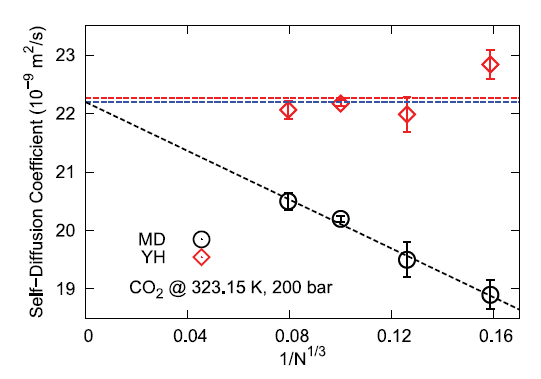
\includegraphics[width=3.2in]{MoultosFig1.png}
	\caption{System size dependence of self-diffusivity obtained with Einstein approach. Reproduced with permission from J. Chem. Phys. 145, 074109 (2016). Copyright 2016 AIP Publishing \cite{Moultos2016}. Blue dashed lines are obtained by extrapolating the MD results to the infinite system size, i.e. $N^{-1/3} \to 0$. Red diamonds are the values of $D$ after correcting for finite size effects, i.e. Equation \ref{eq:YH-correction}. The red dashed line is an average of these corrected values of $D$. For further details, see Ref. \cite{Moultos2016}.}
	\label{fig:MoultosFig1}
\end{figure}


%RAM: This has been moved to the general transport discussion
%Multiple time origins used for MSD (block averaging) - is there a best practice?

%%% I think we agreed that the next secton was covered earlier so I commented it out. -EJM
% \subsubsection{Improved precision} \label{sec:Self-Diffusivity:General:Improved precision}
%
% Compute the diffusion coefficient separately in each dimension, i.e. $D_{xx}$, $D_{yy}$, and $D_{zz}$. For a homogeneous system, $D_{xx}$, $D_{yy}$, and $D_{zz}$ should be equal and provides a useful validation of simulation quality. The variation in these values can be used for a rough estimate of the statistical uncertainty, although more rigorous methods for uncertainty estimation are recommended (see Sec.\ \ref{sec:General: Uncertainty}).

%\begin{enumerate}
%	\item Use ``unwrapped coordinates'' of molecule center of mass to determine mean squared displacement; can also track all atomic coordinates and ensure consistency with center of mass.
%	%Does ``unwrapped coordinates'' require an explanation? Do most open-source simulation packages have the option to track ``unwrapped coordinates''? -ramess101
%	\item Finite size effects tend to be significant and need to be accounted for, i.e. system size corrections must be applied. For example, see \cite{Yeh2004,Moultos2016}. Some correction approaches require that the viscosity be calculated first or that multiple simulations are run with varying box sizes / number of molecules in order to estimate the infinite size limit of the self-diffusivity.
%	\item Multiple time origins used for MSD (block averaging) - is there a best practice?
%	\item Compute the diffusion coefficient separately in each dimension, i.e. $D_{xx}$, $D_{yy}$, and $D_{zz}$. For a homogeneous system, $D_{xx}$, $D_{yy}$, and $D_{zz}$ should be equal and provides a useful validation of simulation quality. The variation in these values can be used for a rough estimate of the statistical uncertainty, although more rigorous methods for uncertainty estimation are recommended (see item \ref{item:uncertainty}).
%\end{enumerate}

\subsection{Self-Diffusivity: Einstein} \label{sec:Self-Diffusivity Einstein}

%I think that we should have this just as a general Einstein approach section and then if anything is specific to Self-Diffusivity we move it to a new section -ramess101

\subsubsection{Output frequency} \label{sec:Self-Diffusivity:Einstein: Output frequency}

Self-diffusivities are computed by post-processing a trajectory. For the Einstein self-diffusivity, this means the positions of the atoms (or molecule centers of mass) should be stored as a function of time so that the MSD can be computed. How often should one save positions and at what frequency? There will always be a trade-off between accuracy (which argues for more configurations saved more frequently) and file size or runtime performance (both of which argue for fewer configurations saved less frequently). Since the long-time slope in MSD is required in the Einstein approach, configurations do not need to be saved at a high frequency. As a general guideline, to balance file size and accuracy, we recommend that approximately 1000 independent configurations be saved at uniform time intervals over the length of a production run.

\subsubsection{Simulation length} \label{sec:Self-Diffusivity:Einstein: Simulation length}

Simulation length needed depends on number of molecules for which transport properties are desired. Fewer molecules requires more simulation time and vice versa. %RAM: Is this a general statement, or just specific to self-diffusivity and Einstein?
Regardless, the simulation must be long enough so that the molecules are in the diffusive regime. We recommend computing the slope from a log-log plot of MSD with respect to time, which should be approximately 1 in the diffusive regime (see Figure \ref{fig:KondratyukFig2}). As mentioned in Section \ref{sec:General: Common pitfalls}, another heuristic is whether the MSD is sufficiently large, i.e. larger than the square of the radius of gyration of the molecule at the low end and larger than the square of half the box length at the high end. If these criteria are met, then one can have confidence that the diffusive regime has been sampled.

% and computing the slopeThe slope should be approximately 1 for a log-log plot of MSD with respect to time
% One way of checking this is to create a log-log plot of MSD with respect to time . In the diffusive regime the slope of a log-The slope should be around 1. if the slope of a log-log plot of MSD vs. t = 1

\subsubsection{Data analysis} \label{sec:Self-Diffusivity:Einstein: Data analysis}

In order to obtain reliable estimates of $D$, it is important to consider how the linear regression is performed for the MSD with respect to time (Equation 2). Specifically, the time interval that is included in the regression can have a significant impact on the predicted value of $D$. We recommend that only the ``middle'' of the MSD be used in the fit. Short time must be excluded as it follows a ballistic trajectory, while very long time is excluded due to the increased noise. Currently, we are unaware of an objective approach for defining the ``middle'' region. Until such an approach exists, we recommend that the author reports how the region was selected and how much variability in $D$ can be attributed to the choice of this region. In addition, the uncertainty in the fit of the slope should be reported. A typical plot, borrowed from Ref. \cite{Kondratyuk2016}, is provided in Figure \ref{fig:KondratyukFig2}, where the linear regressions at long time are included.

%What about when the middle region is subdiffusive like in Figure \ref{fig:KondratyukFig2}?
%How do you fit the MSD (what time interval do you use?) Short time is ballistic trajectory; very long time you get noise, so you need to fit to the “middle” of the MSD. We need to define protocols for how to objectively define this. You should compute the uncertainty in the fit of the slope. Report how the line was fit and associated variables. Is there literature on this? We need to come up with a recommendation for how to do this objectively and consistently.
% If there is no published literature on the subject, rather than provide a recommendation, should we just present the issue that they need to be aware of? -ramess101
% I think we should have a figure to help visualize this -ramess101

\begin{figure}[htb!]
	\centering
	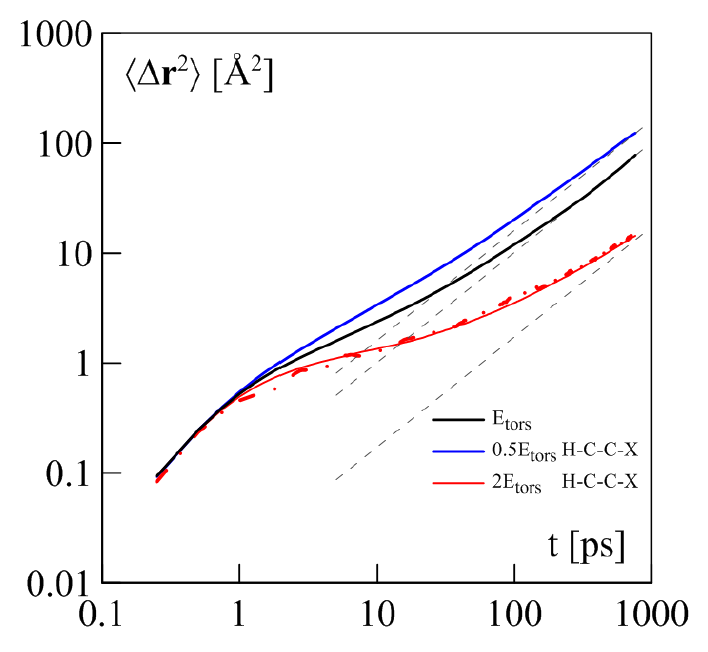
\includegraphics[width=3.2in]{KondratyukFig2.png}
	\caption{Log-log plot of MSD with respect to time. Reproduced with permission from J. Phys. Conf. Ser. 774 (2016) 012039, under the Creative Commons Attribution 3.0 license \cite{Kondratyuk2016}. The gray dashed lines are the long-time asymptotes of the MSD, as determined by the authors. For further details, see Ref. \cite{Kondratyuk2016}.}%The color for each line corresponds to different torsional force field parameters. The red dash-dot line shows the LAMMPS averaging methodology.
	\label{fig:KondratyukFig2}
\end{figure}

%\subsubsection{Uncertainty}
%
%Compute statistical uncertainty by running independent replicates (using multiple starting states from $NPT$ run at desired temperature) and taking the standard deviation (what do the uncertainty people say?) How many replicates do we recommend? \label{item:uncertainty}


%\begin{enumerate}
%    \item Output frequency should be sufficient to have around 1000 data points over the entire MSD. Typical recommendations are every NEED RECOMMENDATION
%	\item In order to obtain reliable estimates of D, it is important to consider how the linear regression is performed for the MSD with respect to time (Equation 2). Specifically, the time interval that is included in the regression can have a significant impact on the predicted value of D. We recommend that only the “middle” of the MSD be used in the fit. Short time must be excluded as it follows a ballistic trajectory, while very long time is excluded due to the increased noise. Currently, we are unaware of an objective approach for defining the “middle” region. Until such an approach exists, we recommend that the author reports how the region was selected and how much variability in $D$ can be attributed to the choice of this region. In addition, the uncertainty in the fit of the slope should be reported.
%	What about when the middle region is subdiffusive like in Figure \ref{fig:KondratyukFig2}?
%	%How do you fit the MSD (what time interval do you use?) Short time is ballistic trajectory; very long time you get noise, so you need to fit to the “middle” of the MSD. We need to define protocols for how to objectively define this. You should compute the uncertainty in the fit of the slope. Report how the line was fit and associated variables. Is there literature on this? We need to come up with a recommendation for how to do this objectively and consistently.
%	% If there is no published literature on the subject, rather than provide a recommendation, should we just present the issue that they need to be aware of? -ramess101
%	% I think we should have a figure to help visualize this -ramess101
%	\item Simulation length needed depends on number of molecules for which transport properties are desired. Fewer molecules requires more simulation time and vice versa. Regardless, the simulation must be long enough so that the molecules are in the diffusive regime. One way of checking this is if the slope of a plot of ln(MSD) vs ln (t) = 1. Other heuristics are: is the MSD sufficiently large (larger than the square of the radius of gyration of the molecule at the low end, and larger than the square of half the box length at the high end).
%	\item Compute statistical uncertainty by running independent replicates (using multiple starting states from $NPT$ run at desired temperature) and taking the standard deviation (what do the uncertainty people say?) How many replicates do we recommend? Link to Sampling/Uncertainty doc. Use Zwanzig/Szabo four-time correlation for MSD averaging…. \label{item:uncertainty}
%\end{enumerate}

%RAM: I do not think that we need to talk about force field accuracy
%FYI: Richard Elliot I developed a database for self-diffusivity that covered all experimental data from the literature as far as he could find. It is included as supporting information in Ind. Eng. Chem. Res. 2010, 49, 3411–3423. This paper provides a generalized correlation of the quantity rho*D (g/cm-s) of n-alkanes at all molecular weights, temperatures, and densities below the entanglement threshold. This semi-empirical correlation is used as the basis for correlating non-alkanes as well. Accuracy diminished for associating compounds, but experimental data were relatively few in number for associating compounds.

\subsection{Self-Diffusivity: Green-Kubo} \label{sec:Self-Diffusivity Green-Kubo}

%Many of the same best practices for the Einstein approach apply to the Green-Kubo method. Specifically, items 1, 2, 4, 5, 6, 7, and 12 from the previous Section are also applicable to the Green-Kubo approach. Some key differences are:

\subsubsection{Output frequency} \label{sec:Self-Diffusivity:Green-Kubo: Output frequency}

If the self-diffusivity is computed using a Green-Kubo approach, the velocities are needed as a function of time. Note that compared to the position information required by the Einstein approach, velocity information must be stored at a much higher frequency for the Green-Kubo approach. This is because the velocity autocorrelation function (VACF) that must be integrated decays very rapidly and fine time resolution is needed to perform an accurate numerical integration.  We recommend saving the velocities at least every 4-5 fs. Be warned that this will result in trajectories that are significantly larger than positional trajectories saved at lower frequencies.

\subsubsection{Simulation length} \label{sec:Self-Diffusivity:Green-Kubo: Simulation length}

Simulations should be long enough that the Green-Kubo integral has reached a plateau. Note that the plateau time is not the same as the required simulation time, since multiple time origins $(t_0)$ are used to compute the Green-Kubo integral.

\subsubsection{Data analysis} \label{sec:Self-Diffusivity:Green-Kubo: Data analysis}

The most common method for computing the self-diffusivity from the VACF is to do a direct numerical integration of the VACF. If this is done, the author should provide details on how the integration was carried out (numerical procedure, algorithm, cutoffs, etc.). The running integral versus time is calculated and the self-diffusivity is estimated from the plateau value. Note that when calculating the VACF, the maximum lag taken should be up to half the total simulation time since longer times serve to increase statistical noise. Also, note that the long time "tail" of the VACF must be properly converged as it contributes significantly to the integral. Like with the MSD, a cut-off needs to be determined when deciding when the integral has converged. It is important to report how sensitive the estimate is to this cut-off time. 
%RAM: I feel like this is unnecessary, since we already discuss in the introduction that both D and eta can be computed using either Einstein or Green-Kubo
%Note that this procedure shares many features to computing the shear viscosity via a Green-Kubo approach; more details are provided in Section~\ref{sec:Viscosity:Green-Kubo: Data analysis}.

%\subsubsection{Uncertainty}
%
%Independent simulations should be run and each integral can be averaged together to obtain a smoothed integral. With these replicate simulations, we recommend that the uncertainty be determined using a bootstrap methodology:
%	\begin{enumerate}
%		\item Randomly selecting (with replacement) from the set of replicate simulations
%		\item Calculating the average integral from this random set
%		\item Computing the self-diffusivity
%		\item Repeat steps a)-c) thousands of times
%		\item Generate distribution of the estimated values of self-diffusivity
%		\item Compute uncertainty by integrating distribution at desired confidence level
%	\end{enumerate}

%\begin{enumerate}
%	\item Need to write velocities instead of positions, and the frequency should be much higher because the integral of the velocity autocorrelation function decays rapidly. Recommend writing every 5 fs.
%	\item Integrate the VACF numerically, providing details of how this is done.
%	\item Plot the running integral vs time. The data are best at short-time and noise takes over at long times. Like with the MSD, a cut-off needs to be determined when you decide the integral has converged. It is important to report how sensitive the estimate is to this cut-off time. \label{item:GreenKuboDiffusivity}
%	\item Independent simulations should be run and each integral can be averaged together to obtain a smoothed integral. With these replicate simulations, we recommend that the uncertainty be determined using a bootstrap methodology:
%	\begin{enumerate}
%		\item Randomly selecting (with replacement) from the set of replicate simulations
%		\item Calculating the average integral from this random set
%		\item Estimating the self-diffusivity as described in item \ref{item:GreenKuboDiffusivity}
%		\item Repeat steps a)-c) thousands of times
%		\item Generate distribution of the estimated values of self-diffusivity
%		\item Compute uncertainty by integrating distribution at desired confidence level
%	\end{enumerate}
%\end{enumerate}

\subsection{Self-Diffusivity: Special topics} \label{sec:Self-Diffusivity Special topics}

Although molecular simulation is well-suited for predicting diffusivity coefficients in membranes, several issues arise that require special attention. For example, the standard non-bonded long-range cut-off corrections are not straightforward in a heterogeneous system. For this reason, it is common to modify the non-bonded interactions such that tail corrections are not needed, e.g. cut-and-shift, force-switch \cite{GROMACS,Brooks2009}. However, it is important to investigate the impact modifying the non-bonded potential has on the diffusion coefficients. Furthermore, since membranes require anisotropic pressure control it is important to use barostats/thermostats that maintain the correct isobaric/isothermal ensemble. Venable et al. have shown that as long as a high-quality barostat and thermostat are used (such as those implemented via so-called "extended system" methods \cite{Nose1984,Hoover1985}), diffusion constants determined from NVE and NPT simulations are quite similar \cite{Venable2017}. Finally, correcting diffusion coefficients for finite size effects (i.e. when periodic boundary conditions are employed) in membrane systems requires some additional consideration. Camley et al. developed a method for determining diffusion constants in membrane systems which uses the immersed-boundary approach in the context of the the Saffman-Delbr{\"u}uck model \cite{Camley2015}. This method is available via \url{https://diffusion.lobos.nih.gov}.

%For systems that require anisotropic pressure control (e.g. membranes, etc.), use of a barostat/thermostat that maintains the correct isothermal/isobaric ensemble (e.g. extended system, Langevin piston) is required.

%Calculating diffusion in membrane systems with periodic boundary conditions require some additional consideration, e.g. Saffman-Delbruck model \cite{Camley2015,Venable2017}.

%The standard non-bonded long-range cut-off corrections are not straightforward when computing diffusivity in a heterogeneous system.

%Handling potential truncation: shifted force, shifted potential, cutoff, long range corrections. We need to come up with recommendations on this.

%\begin{enumerate}
%	\item Calculating diffusion in membrane systems with PBC require some additional consideration, use of Saffman-Delbruck model: see http://pubs.acs.org/doi/abs/10.1021/acs.jpcb.6b09111, also http://dx.doi.org/10.1063/1.4932980
%	\item For systems that require anisotropic pressure control (e.g. membranes etc), use of a barostat/thermostat that maintains the correct isothermal/isobaric ensemble (e.g. extended system, Langevin piston) is required.
%	\item Handling potential truncation: shifted force, shifted potential, cutoff, long range corrections. We need to come up with recommendations on this.
%\end{enumerate}

\section{Viscosity} \label{sec:Viscosity}

%Similar to self-diffusivity, EMD for viscosity is straightforward but its reliability compared to experimental data has not been evaluated with a comprehensive database. Many more experimental data are available for viscosity than for self-diffusivity. Anecdotal studies with small databases show encouraging results, but deviations from experiment can range from 5-35\% even when results are said to be “good.” Nieto-Draghi et al. provide a useful review of the status quo \cite{Nieto2015}. EMD may deviate 2x more than NEMD from experimental data; hydrogen bonding throws in complications that may require empirical corrections.

% I don't think we want to talk about comparison to experimental data. We are not really concerned about if diffusivity or viscosity are accurately predicted relative to experiment, we just want to present the best methods for obtaining reproducible/honest results. In addition, you can predict viscosity more accurately if you parameterize your force field for such a purpose. -ramess101

% I am unaware of this - can a citation be given? -ejmaginn

Although the popularity of NEMD methods for predicting viscosity has increased in recent years, Ref. \cite{Chen2009} demonstrates that EMD methods can be of equal accuracy and reliability to NEMD as long as best practices are followed, i.e. proper system set-up and thorough data analysis. That being said, EMD works best for fluids with relatively low viscosity, i.e. typically less than 20 cP although EMD has been successfully implemented for systems near 50 cP. Higher viscosity systems are extremely difficult to compute with EMD and so NEMD methods are often preferred in this case.

The recommended EMD approach for predicting viscosity is Green-Kubo. The Green-Kubo approach appears to be the most popular EMD method found in the literature and, more importantly, less arbitrary data analysis methods exist that improve the reliability and reproducibility (see Sec. \ref{sec:Viscosity:Green-Kubo: Data analysis}). 

We should note, however, that Ref. \cite{Hess2002} states that the Einstein relation is more convenient than Green-Kubo for viscosity because ``inaccuracies in the long-time correlations can be ignored by only considering integral over shorter times.'' 
%What do we want to make of this claim? -RAM
Although this observation is true (see Figure \ref{fig:Einstein_3terms_30replicates}), several algorithmic advances have been implemented with the Green-Kubo approach since 2002 (when Ref. \cite{Hess2002} was published). Most of these improvements rely on performing large amounts of replicate simulations (see Sec. \ref{sec:Viscosity:General: Improved precision}). Therefore, we only recommend utilizing the Einstein approach when replicate simulations are too computationally expensive (see Sec. \ref{sec:Viscosity:Einstein: Data analysis}).  

%The recommended EMD approach for predicting viscosity is Green-Kubo. We should note that Ref. \cite{Hess2002} claims that the Einstein relation is more convenient than Green-Kubo for viscosity because ``inaccuracies in the long-time correlations can be ignored by only considering integral over shorter times.'' 
%%What do we want to make of this claim? -RAM
%As discussed in Sec. , this advantage is primarily of 
%However, several algorithmic advances (see Sec. \ref{sec:Viscosity:Green-Kubo: Data analysis}) have been implemented with the Green-Kubo approach since 2002 (when Ref. \cite{Hess2002} was published). As discussed in Sec. \ref{sec:Viscosity:General: Improved precision}, these improvements rely on performing large amounts of replicate simulations, which is now more computationally feasible. For these reasons, the Green-Kubo approach now appears to be the most popular EMD method found in the literature. More importantly, less arbitrary data analysis methods exist that improve the reliability and reproducibility (see Sec. \ref{sec:Viscosity:Green-Kubo: Data analysis}).

%The recommended EMD approach for predicting viscosity is Green-Kubo. We should note that Hess claims that the Einstein relation is more convenient than Green-Kubo for viscosity because ``inaccuracies in the long-time correlations can be ignored by only considering integral over shorter times.'' \cite{Hess2002}
%%What do we want to make of this claim? -RAM
%However, several advances have been implemented with the Green-Kubo approach since 2002 (when Ref. \cite{Hess2002} was published). The Green-Kubo approach now appears to be the most popular EMD method found in the literature. More importantly, less arbitrary data analysis methods exist that improve the reliability and reproducibility (see Sec. \ref{sec:Viscosity:Green-Kubo: Data analysis}).

Section \ref{sec:Viscosity General} discusses shear viscosity checklist items that apply to both the Einstein and Green-Kubo approaches. Sections \ref{sec:Viscosity Green-Kubo} and \ref{sec:Viscosity Einstein} discuss checklist items specific to the Green-Kubo and Einstein approaches, respectively, for estimating viscosity. Section \ref{sec:Viscosity Special topics} provides a brief discussion of some topics that are relevant in certain applications.


\subsection{Viscosity: General} \label{sec:Viscosity General}

\subsubsection{Simulation length} \label{sec:Viscosity:General: Simulation length}

Overall you need about 10X more data to compute viscosity than diffusivity, since viscosity is a collective property. As with the self-diffusivity, the simulation time needs to be long enough so that all the relaxation processes are adequately sampled. We recommend applying similar heuristics as those described in Section~\ref{sec:General: Common pitfalls} to determine the length of the simulation required.

Figure \ref{fig:ZhangFig8}, borrowed from Ref. \cite{Zhang2015}, demonstrates that if the length of each independent trajectory is too short the viscosity will not converge to the correct value, regardless of how many replicates are used. Specifically, the average viscosity obtained from 100 replicates of 500 ps appears to diverge from the 1, 2, and 4 ns simulation results, suggesting that 500 ps is not sufficiently long for this system. Since it is very hard to know how long an individual trajectory needs to be, we recommend performing an analysis similar to that shown in Figure~\ref{fig:ZhangFig8} to ensure adequate sampling.

\begin{figure}[htb!]
	\centering
	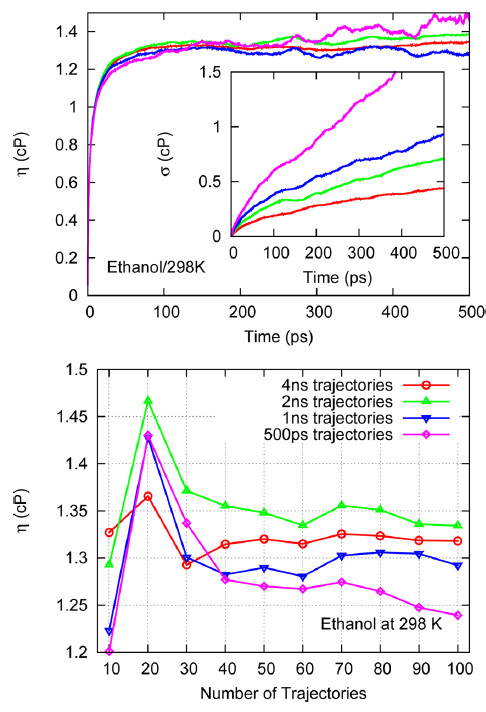
\includegraphics[width=3.2in]{ZhangFig8.png}
	\caption{Viscosity dependence on simulation length. Reprinted with permission from J. Chem. Theory Comput., 2015, 11 (8), pp 3537–3546. Copyright (2015) American Chemical Society Ref.\ \cite{Zhang2015}. Different lines and symbols correspond to different simulation length, i.e. trajectory time. The inset in the top panel plots the standard deviation, $\sigma$. For further details, see Ref. \cite{Zhang2015}.}
	\label{fig:ZhangFig8}
\end{figure}

It is important not to confuse the Green-Kubo integration time (the abscissa for the top panel of Figure \ref{fig:ZhangFig8}) with the simulation length (the different color lines in both panels of Figure \ref{fig:ZhangFig8}). Recall that the Green-Kubo integral (plotted in the top panel) is evaluated using multiple time origins $(t_0)$, so the Green-Kubo integral contains more independent trajectories for the 4 ns line than the 500 ps line. Therefore, the time at which the Green-Kubo integral reaches a plateau (around 100 ps in the top panel of Figure \ref{fig:ZhangFig8}) is not the same as the required simulation time. For sufficient independent trajectories, the required simulation time should typically be around an order of magnitude greater than the plateau time.

Figure \ref{fig:ZhangFig10}, borrowed from Ref. \cite{Zhang2015}, demonstrates that the plateau time increases with increasing viscosity, where an order of magnitude increase in viscosity corresponds to approximately an order of magnitude increase in the plateau time. In order to account for the increase in the plateau time, higher viscosity fluids require longer overall simulation times.

\begin{figure}[htb!]
	\centering
	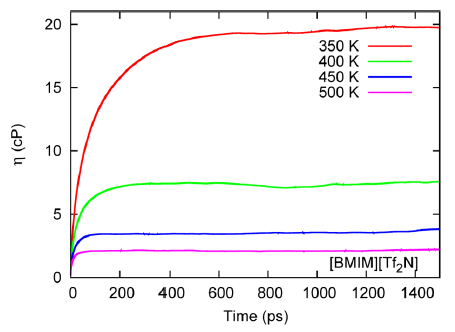
\includegraphics[width=3.2in]{ZhangFig10.png}
	\caption{Plateau time dependence on viscosity. Reprinted with permission from J. Chem. Theory Comput., 2015, 11 (8), pp 3537–3546. Copyright (2015) American Chemical Society Ref.\ \cite{Zhang2015}. Different lines correspond to different temperatures and, thus, different viscosities. For further details, see Ref. \cite{Zhang2015}.}
	\label{fig:ZhangFig10}
\end{figure}

% we recommend that a longer overall simulation length should also increase with increasing viscosity.

% Since the overall simulation length should reflect this increase in the plateau region, . Note that the dependence of plateau time on viscosity is roughly linear  plateau time If the plateau time of 500 K and 350 K are approximated as 80 ps and 800 ps, respectively, and the corresponding v

\subsubsection{Output frequency} \label{sec:Viscosity:General: Output frequency}

As with the self-diffusivity, shear viscosity is computed by post processing a data file. If the Green-Kubo procedure is used, stress tensor components need to be written out frequently enough so that an accurate estimate of the time integral can be made. Since the integral decays quickly with time, we recommend writing the stress tensor every 5 to 10 fs. If the Einstein relationship is used, less frequent writes can be made over the length of the simulation. The user should perform some preliminary tests to ensure write frequencies are sufficient as well as to estimate file sizes for a given simulation.

\subsubsection{Finite size effects} \label{sec:Viscosity:General: Finite size}

Figures \ref{fig:MoultosFig3}-\ref{fig:ZhangFig9} from Refs. \cite{Moultos2016} and \cite{Zhang2015}, respectively, suggest that finite size effects are not significant for systems with as few as 125 and 500 molecules, respectively. Other authors, including Daivis and Evans \cite{Daivis:1995}, have also reported that shear viscosity has a weak dependence on system size (see Figure 4 of Ref. \cite{Daivis:1995}). It is thus reasonable to neglect a system size correction, although if possible we recommend that users carry out some additional calculations to justify this assumption. 

To test for system size dependence, one can run a series of simulations over a range of $N$ molecules, where $N$ is varied at least by a factor of two and ideally an order of magnitude. By plotting the computed shear viscosity versus $N^{-1/3}$, it is possible to ascertain if there are system size effects. We encourage authors to report these findings to help further verify system size effect trends on viscosity.  If a linear trend is observed with respect to $N^{-1/3}$, the infinite system size viscosity can be extrapolated as the intercept from a linear regression. The author should report the uncertainty associated with this linear fit and extrapolation.
% Should we recommend how much to vary the system size? In other words, varying the size from 200 to 250 is probably not very informative. But varying the size from 200 to 400 to 800 to 1600 will probably show you if there is a trend. So should we recommend "several" different system sizes that vary by a factor of 2 or greater? Also, normally the plot has 1/N^(some power) as the horizontal axis, where the power might have a theoretical value. These plots are nice since N=infinity corresponds to the vertical axis. I think we should mention this. -ramess101

\begin{figure}[htb!]
	\centering
	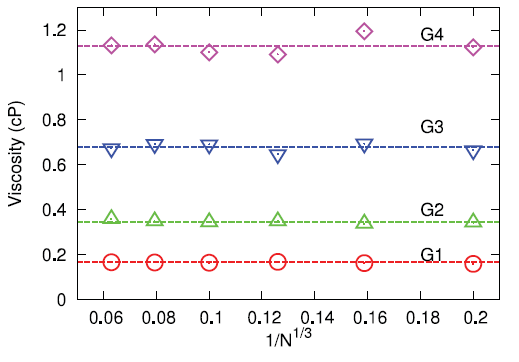
\includegraphics[width=3.2in]{MoultosFig3.png}
	\caption{Finite size effects for viscosity obtained with Green-Kubo approach. Reproduced with permission from J. Chem. Phys. 145, 074109 (2016). Copyright 2016 AIP Publishing \cite{Moultos2016}.  Different symbols correspond to different types of glymes (Gi). Dashed lines are average value for each glyme from various system sizes $(N)$. For further details, see Ref. \cite{Moultos2016}.}
	\label{fig:MoultosFig3}
\end{figure}

\begin{figure}[htb!]
	\centering
	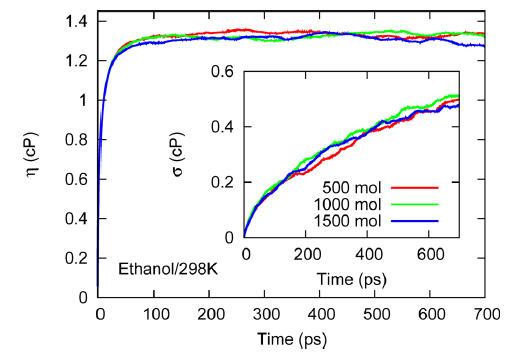
\includegraphics[width=3.2in]{ZhangFig9.png}
	\caption{Finite size effects for viscosity obtained with Green-Kubo approach. Reprinted with permission from J. Chem. Theory Comput., 2015, 11 (8), pp 3537–3546. Copyright (2015) American Chemical Society  Ref. \cite{Zhang2015}. Different colors correspond to different number of molecules. The inset plots the standard deviation, $\sigma$. For further details, see Ref. \cite{Zhang2015}.}
	\label{fig:ZhangFig9}
\end{figure}

\subsubsection{Improved precision}	\label{sec:Viscosity:General: Improved precision}

To improve statistical averaging, it is common to include multiple terms from the stress tensor. For example, Figure \ref{fig:HessFig5}, borrowed from Ref. \cite{Hess2002}, demonstrates the improvement of averaging the three off-diagonal elements of the pressure tensor, compared to a single off-diagonal element. To maximize simulation efficiency for an isotropic system, we recommend that users employ a generalized form of the Green-Kubo integral \citep{Evans:90, Daivis:1994}, which uses all six independent components of the stress tensor. Details are given in the Appendix of Ref. \cite{Daivis:1994}. This generalized integral is given by
\begin{equation}
  \eta = \frac{V}{10 k_B T}  \int_0^\infty \left\langle \tau_{ij}^{os}(0)\tau_{ij}^{os}(t) \right\rangle_{t_0} dt
  \label{eq:GKwonder}
\end{equation}
where the components $\tau_{ij}^{os}$ of the traceless, symmetric part of the stress tensor are given by
\begin{equation}
  \tau_{ij}^{os} = \frac{\tau_{ij}+\tau_{ji}}{2} - \delta_{ij} \left( \frac{1}{3} \sum_k \tau_{kk} \right)
  \label{eq:Pwonder}
\end{equation}
where $\delta$ is the unit tensor. Note that the factor of 10 in the denominator of Eq.~\ref{eq:GKwonder} results from assigning weighting factors of 3/3 and 4/3 for each of the six off-diagonal terms and the three diagonal terms, respectively \cite{Liu2012,Borodin2009,Mondello1997} (although some authors have argued for an equal weighting \cite{Chen2009}, which would modify the normalization factor in the denominator of Eq.~\ref{eq:GKwonder}).
% from a 3/3 contribution from each of the six off-diagonal terms plus an implicit 4/3 contribution from each of the three diagonal terms. 
The equivalent generalization of the Einstein relation is
\begin{equation}
  \eta = \frac{V}{20 k_B T} \lim_{t\to\infty} \frac{d}{dt} \sum_i \sum_j \left\langle \int_0^t \tau_{ij}^{os}(t') dt' \right\rangle_{t_0}
  \label{eq:Einwonder}
\end{equation}

We are not aware of any studies that rigorously quantify the improvement in precision obtained by using all six terms. Figure \ref{fig:ChenFig1}, borrowed from Ref. \cite{Chen2009}, demonstrates that the average viscosity and fluctuations are nearly identical when using the three off-diagonal terms or when using six terms. Therefore, although we recommend including all six terms, it is typically sufficient to utilize just the three off-diagonal terms. Regardless, it is important to clearly state which terms are included when computing viscosity.

\begin{figure}[htb!]
	\centering
	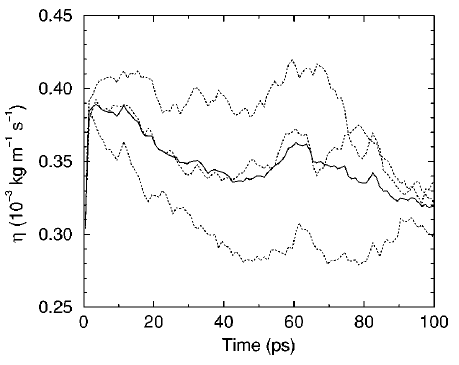
\includegraphics[width=3.2in]{HessFig5.png}
	\caption{Green-Kubo viscosity plot. Reproduced from J. Chem. Phys., 2002, 116(1):209--217, with the permission of AIP Publishing \cite{Hess2002}. Dashed lines represent a single off-diagonal element of the pressure tensor while solid line is the average of the three off-diagonal elements. For further details, see Ref. \cite{Hess2002}.}
	\label{fig:HessFig5}
\end{figure}

\begin{figure}[htb!]
	\centering
	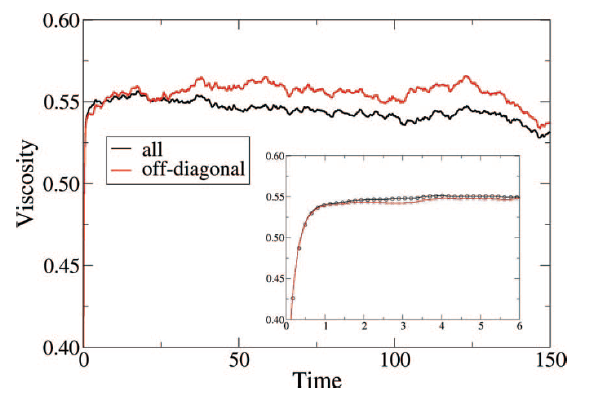
\includegraphics[width=3.2in]{ChenFig1.png}
	\caption{Green-Kubo dimensionless viscosity plot for Lennard-Jones fluid. Reproduced from J. Chem. Phys., 131, 246101 (2009), with the permission of AIP Publishing \cite{Chen2009}. Red line is obtained by averaging the three off-diagonal elements while the black line is obtained from all six pressure tensor elements. For further details, see Ref. \cite{Chen2009}.}
	\label{fig:ChenFig1}
\end{figure}

Although fluctuations in $\eta$ are significantly reduced by including multiple terms from the stress tensor, the key to improved precision of viscosity estimates is to average several replicate simulations. For $N_{\rm reps}$ replicates, the Green-Kubo equation is
\begin{equation}
\eta = \frac{V}{10 k_B T N_{\rm reps}} \sum_{n=1}^{N_{\rm reps}}  \int_0^\infty \left\langle \tau_{ij,n}^{os}(0)\tau_{ij,n}^{os}(t) \right\rangle_{t_0} dt
\label{eq:GKwonder_replicates}
\end{equation}
and the Einstein relation becomes
\begin{equation}
\eta = \displaystyle \frac{V}{20 k_B T N_{\rm reps}} \lim_{t\to\infty} \frac{d}{dt} \sum_{n=1}^{N_{\rm reps}} \sum_i \sum_j \left\langle \int_0^t \tau_{ij,n}^{os}(t') dt' \right\rangle_{t_0}
\label{eq:Einwonder_replicates}
\end{equation}

For example, Figure \ref{fig:Einstein_3terms_30replicates} demonstrates that averaging three stress tensors is not sufficient to obtain a reliable Einstein slope as $t \to \infty$. By contrast, a near linear trend at high time is observed by averaging a large number (30) of replicates.

\begin{figure}[htb!]
	\centering
	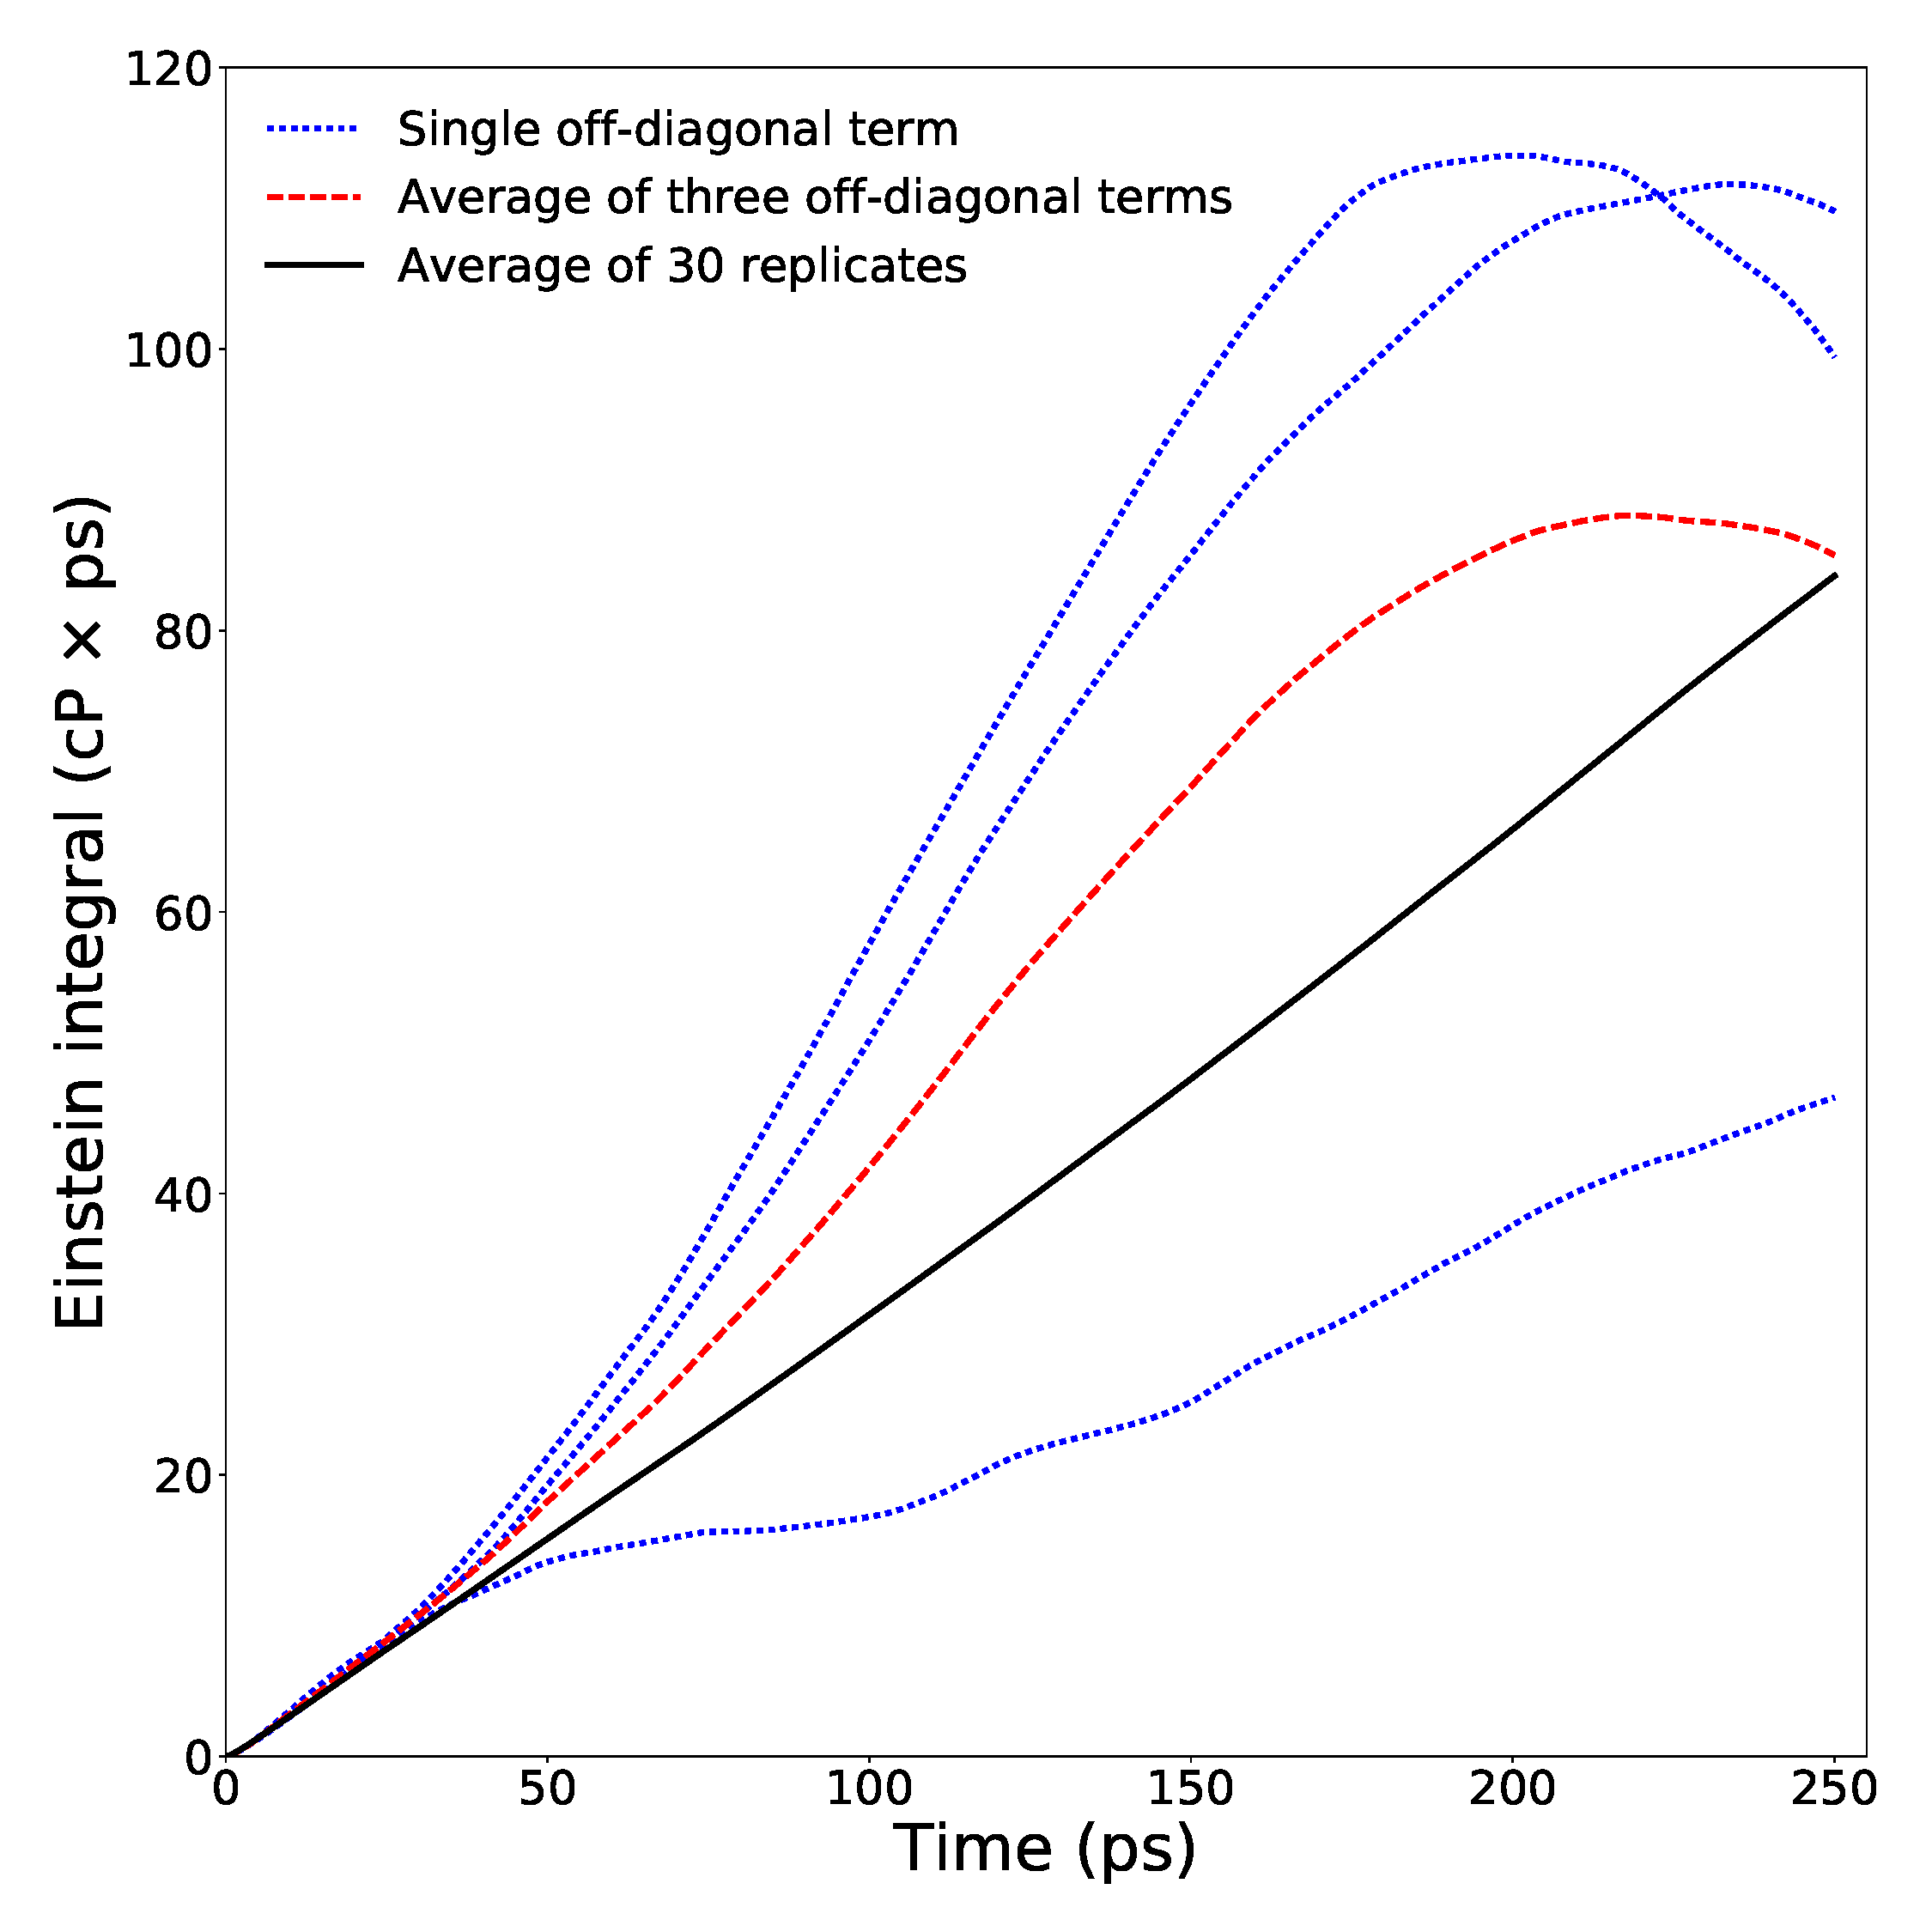
\includegraphics[width=3.2in]{Einstein_3terms_30replicates.pdf}
	\caption{Improvement with three stress tensor terms and 30 replicate runs. Simulations were performed with Gromacs 2018 for saturated liquid ethane at 137 K using the TraPPE-UA model \cite{Martin1998}. Simulation details: velocity Verlet integrator, 2 fs time-step, 6 fs pressure tensor output frequency, 12 time origins, 1 ns equilibration time, 1 ns production time, 400 molecule system, 1.4 nm non-bonded cut-off distance with analytic tail corrections, Nos{\'e}-Hoover thermostat with time constant of 1 ps, bond-lengths constrained with LINCS algorithm \cite{GROMACS}.}
	\label{fig:Einstein_3terms_30replicates}
\end{figure}

The number of replicates used in the literature varies widely. In their study of the shear viscosity of alkanes, Payal and co-workers \cite{Payal2012} used 10 replicates, whereas Zhang et al. \cite{Zhang2015} performed a systematic investigation of the minimal number of replicates required for convergence. They observed that a value of 30 to 40 replicates was statistically equivalent to 100 replicates for their system. However, the necessary number of replicates depends on the system. Specifically, the compound, the temperature, the number of molecules, and the simulation time all influence the optimal number of replicates. We recommend that researchers plot how $\eta$ varies with respect to the number of replicates for a range of 10 to 30 replicates to determine if additional simulations are needed.

%\begin{enumerate}
%	\item Simulation length: overall you need about 10X more data to compute viscosity than diffusivity, since viscosity is a collective property. Also requires sufficient simulation time for “4-5 molecular rotations” on average.
%	% Do we have any literature to support this? -ramess101
%	\item Output frequency should be high (every 5-10 fs); this needs to be checked for the particular system.
%	\item Finite size effects: Figures \ref{fig:MoultosFig3}-\ref{fig:ZhangFig9} from \cite{Moultos2016} and \cite{Zhang2015}, respectively, suggest that finite size effects are not significant for systems with as few as 125 and 500 molecules, respectively. More work needs to be done to verify this. We recommend that users look for system size effects by plotting the viscosity with respect to $N^{-1/3}$, where $N$ is the number of molecules. The range of $N$ should span an order of magnitude or, if this is computationally intractable, at least a factor of two. The author should report any dependence observed for viscosity with respect to system size. If a linear trend is observed with respect to $N^{-1/3}$, the infinite system size viscosity can be extrapolated as the intercept from a linear regression. The author should report the uncertainty associated with this linear fit and extrapolation.
%	% Should we recommend how much to vary the system size? In other words, varying the size from 200 to 250 is probably not very informative. But varying the size from 200 to 400 to 800 to 1600 will probably show you if there is a trend. So should we recommend "several" different system sizes that vary by a factor of 2 or greater? Also, normally the plot has 1/N^(some power) as the horizontal axis, where the power might have a theoretical value. These plots are nice since N=infinity corresponds to the vertical axis. I think we should mention this. -ramess101
%	\item To improve statistical averaging, we recommend using all six of the symmetrized traceless stress tensor terms. Figure \ref{fig:ChenFig1}, taken from \cite{Chen2009}, demonstrates that the viscosity is nearly identical when using the three off-diagonal terms or when using six terms.
%\end{enumerate}





\subsection{Viscosity: Green-Kubo} \label{sec:Viscosity Green-Kubo}

%\subsubsection{Improved precision} \label{sec:Viscosity:Green-Kubo: Improved precision}

%To smooth noise in Green-Kubo integral, we recommend performing independent replicate trajectories (i.e. different initial configurations or random seed to initialize velocities). The primary advantage of performing replicates as opposed to one longer simulation is the computational speed-up. Figure \ref{fig:PayalFig2}, taken from Payal et al. \cite{Payal2012}, demonstrates that an average of 10 replicate simulations of 2 ns length converges to the same value as a single 4 ns simulation. Since these replicates can be performed in parallel the computational time is reduced by a factor of two, in this example. However, Figure \ref{fig:ZhangFig8}, taken from \cite{Zhang2015}, demonstrates that if the length of each independent trajectory is too short the viscosity will not converge to the correct value, regardless of how many replicates are used.
%	%\item Averaging over multiple simulations with analytic fitting of integral provides a good way of smoothing noise and provides an objective means of determining the viscosity \cite{Zhang2015}.
%	% I think this point of averaging multiple simulations is important enough to merit its' own discussion
%
%Replicates can provide a more rigorous uncertainty assessment. We recommend bootstrapping the uncertainties by randomly sampling which replicates are included in the average and data analysis procedure (see Green-Kubo for self-diffusivity).

%The number of replicates used in literature varies widely. \cite{Payal2012} somewhat arbitrarily used 10 replicates whereas \cite{Zhang2015} performed a systematic investigation of the minimal number of replicates required for convergence. They observed that a value of 30-40 replicates was statistically equivalent to 100 replicates for their system. However, the necessary number of replicates depends on the system. Specifically, the compound, the temperature, the number of molecules, and the simulation time all influence the optimal number of replicates.

%Furthermore, because the uncertainty is inversely proportional to the square root of the number of replicates (see Figure 7 of \cite{Zhang2015} and Figure 8 of \cite{Ma2017}), increasing the number of replicates is a simple, fast, and direct way to reduce the uncertainty.

\subsubsection{Data analysis} \label{sec:Viscosity:Green-Kubo: Data analysis}

It is imperative to report how the viscosity was estimated from Equation \ref{eq:Green-Kubo}. There are three common methods: average over a specified time interval, fit the autocorrelation function to a model and analytically integrate the model fit, or fit the ``running integral'' to a model and extrapolate the model to infinite time. We recommend the latter methodology but discuss each approach below.

\subsubsection*{Average over time interval}

A slightly ambiguous but common practice is to report an average shear viscosity that is obtained over a specified time interval. Due to large fluctuations at long times, the initial plateau of the integral at short times (around 10 to 100 ps) is typically the region of choice, see Refs. \cite{Fanourgakis2012,Chen2009}. However, it is important to explain how this time interval was selected (i.e. visual inspection, test of convergence, magnitude of fluctuations, etc.) and to quantify how much the estimated viscosity changes if the time interval were modified. For example, in Figures \ref{fig:HessFig5} and \ref{fig:ChenFig1} the reported viscosity would likely be the average from approximately 5 to 15 ps and 10 to 25 dimensionless time units, respectively. Clearly, the estimated viscosity would vary significantly if the long-time data were included in the average. 

\subsubsection*{Model fit to autocorrelation function}

An alternative method is to fit a model to the autocorrelation function before calculating the ``running integral.'' The integral of the model fit can then be evaluated in the limit as $t \to \infty$. This helps to overcome large fluctuations at long times and, thereby, reduces uncertainties. The primary difficulty is finding a model that can adequately match the autocorrelation function without introducing bias into the estimate of viscosity. A common function found in the literature is
\begin{equation} \label{eq:ACF_fit}
\frac{S^{\rm f}_{\rm ACF}(t)}{S^{\rm f}_{\rm ACF}(0)} = (1-C)cos(\omega t)\exp{(-t/\tau_f)^{\beta_f}} + C\exp{(-t/\tau_s)^{\beta_s}}
\end{equation}
where $C, \omega, \tau_f, \tau_s, \beta_f, \beta_s$ (and sometimes $S^{\rm f}_{\rm ACF}(0)$) are fitting parameters. $\omega$ is the frequency of rapid pressure oscillations, $\tau_f$ and $\beta_f$ are the time constant and exponent of fast relaxation in a stretched-exponential approximation, $\tau_s$ and $\beta_s$ are constants for slow relaxation, $C$ is the pre-factor that determines the weight between fast and slow relaxation, $S^{\rm f}_{\rm ACF}(t)$ is the stress autocorrelation function at time $t$, and $S^{\rm f}_{\rm ACF}(0)$ is the initial (time-zero) autocorrelation function \cite{GROMACS}.

%Figure \ref{fig:FanourgakisFig1}, from Ref.  \cite{Fanourgakis2012}, demonstrates that Equation \ref{eq:ACF_fit} can reliably fit the autocorrelation function for this system. However, small deviations in the model fit can lead to significant bias in the estimated viscosity. Similar to the methods discussed previously, it is important to quantify the variability in viscosity that arises from the model fit. For example, we recommend bootstrapping the uncertainties of the model fit. Furthermore, if a weighting function or cut-off time is implemented when fitting Equation \ref{eq:ACF_fit}, the impact of these parameters should be discussed.

Figure \ref{fig:FanourgakisFig1}, from Ref. \cite{Fanourgakis2012}, demonstrates that Equation \ref{eq:ACF_fit} has the correct shape to fit the stress autocorrelation function for this system. However, notice the significant deviation between the model fit $(S^{\rm f}_{\rm ACF})$ and the raw simulation output $(S_{\rm ACF})$ for time less than 0.02 ps and the relatively small deviations in the first two peaks around 0.1 ps. These systematic deviations in the model fit can lead to significant bias in the estimated viscosity. One method to overcome this issue is to place a larger weight on short-time data or to include a cut-off time beyond which $S_{\rm ACF}$ data are not included in the model fit.

\begin{figure}[htb!]
	\centering
	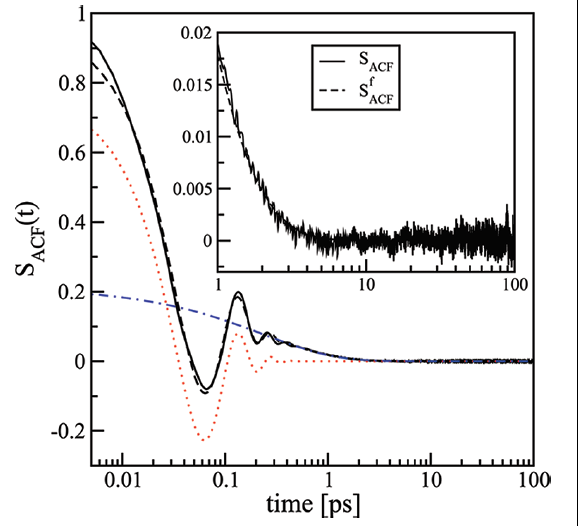
\includegraphics[width=3.2in]{FanourgakisFig1.png}
	\caption{Fit of autocorrelation function to Equation \ref{eq:ACF_fit}. Reproduced with permission from J. Phys. Chem. A., 2012, 116 (10), pp 2564--2570. Copyright (2012) ACS Publications \cite{Fanourgakis2012}. S$_{\rm ACF}$ and S$^{\rm f}_{\rm ACF}$ correspond to the raw autocorrelation function and the fit to Equation \ref{eq:ACF_fit}, respectively. The red dotted line and blue dashed--dotted line correspond to the fast and slow autocorrelation components, respectively, i.e. the first and second terms of Equation \ref{eq:ACF_fit}. For further details, see Ref. \cite{Fanourgakis2012}.}
	\label{fig:FanourgakisFig1}
\end{figure}

%Recall that the main purpose for fitting $S_{\rm ACF}$ to a model (Equation \ref{eq:ACF_fit}) is so that the long-time Green-Kubo integration converges, i.e. so that $S^{\rm f}_{\rm ACF}$ converges to zero as $t \to \infty$. For this reason, it is sometimes preferred to only fit $S_{\rm ACF}$ data after a given time, specifically, after the ``fast'' autocorrelation component has dissipated (the first term in Equation \ref{eq:ACF_fit} and the red dotted line in Figure \ref{fig:FanourgakisFig1}). In other words, the Green-Kubo integration is performed using the raw $S_{\rm ACF}$ simulation output for short time and then $S^{\rm f}_{\rm ACF}$ is used to integrate the Green-Kubo integral to infinite time. 

Alternatively, it is sometimes preferable to integrate the raw $S_{\rm ACF}$ simulation output for short time and then integrate the model fit, $S^{\rm f}_{\rm ACF}$, to infinite time \cite{vanderSpoel1998,Shirts2013,Fernandez2005}. The advantage of this hybrid (combined) integration approach is that the raw data are used in the time region where small deviations in the model fit can lead to large biases in $\eta$, whereas the model fit is utilized in the time region where integration of the raw data does not converge. The hybrid integration approach is especially preferred when $S_{\rm ACF}$ is highly oscillatory, such as that shown in Figure 7 of Ref. \cite{Fernandez2005}, where Equation \ref{eq:ACF_fit} is likely inadequate. 

The time where the Green-Kubo integration switches from using $S_{\rm ACF}$ to $S^{\rm f}_{\rm ACF}$, referred to as the switch-time $(t_{\rm s})$, should be after the ``fast'' autocorrelation component has dissipated (the first term in Equation \ref{eq:ACF_fit} and the red dotted line in Figure \ref{fig:FanourgakisFig1}). As this time depends on the system and user judgment, examples of $t_{\rm s}$ in the literature range widely. For example, $t_{\rm s} = 5$ ps in Refs. \cite{vanderSpoel1998,Shirts2013} while the switch-time value is only 0.015 ps in Ref. \cite{Fernandez2005}.  

A simpler exponential decay function than Equation \ref{eq:ACF_fit} can be used with the hybrid integration approach because the model does not need to fit the autocorrelation function over the entire time range, just for $t > t_{\rm s}$. For example, it is common to fit $S_{\rm ACF}$ values for $t > t_{\rm s}$ to a single exponential term, e.g. $S^{\rm f}_{\rm ACF} = \exp(-(t/\tau)^\beta)$ \cite{vanderSpoel1998}, $S^{\rm f}_{\rm ACF} = \exp(-t/\tau)$ \cite{Shirts2013}, or $S^{\rm f}_{\rm ACF} = a \exp(-t/b)$ \cite{Fernandez2005}, where $\tau$, $\beta$, $a$, and $b$ are fitting parameters. 

%The hybrid integration approach is especially preferred when $S_{\rm ACF}$ is highly oscillatory, such as that shown in Figure \ref{fig:FernandezFig7}, from Ref. \cite{Fernandez2005}. The dashed line in Figure \ref{fig:FernandezFig7} is obtained by fitting the $S_{\rm ACF}$ data (denoted $\Phi_{\eta}(t)$) for $t > 0.015$ ps to the model $S^{\rm f}_{\rm ACF} = a \exp(-t/b)$, where $a$ and $b$ are fitting parameters. Note that a simpler exponential decay function can be used with the hybrid integration approach because the model does not need to fit the autocorrelation function over the entire time range, just for $t > t_{\rm s}$.

%The value of 0.015 ps is referred to as the switch-time, namely, the time where the Green-Kubo integration switches from using $S_{\rm ACF}$ to $S^{\rm f}_{\rm ACF}$. 

%\begin{figure}[htb!]
%	\centering
%	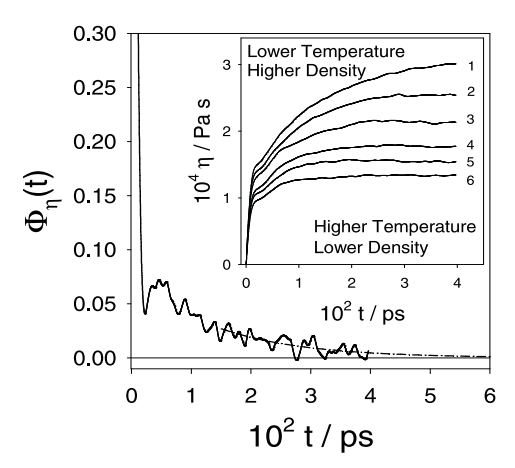
\includegraphics[width=3.2in]{FernandezFig7.png}
%	\caption{Fit of autocorrelation function ($\Phi_{\eta}(t)$) to $a \exp(-t/b)$. Copied from Figure 7 of Ref. \cite{Fernandez2005}. Solid line is the raw autocorrelation function while the dashed line is the model fit for $t > 0.015$ ps. For further details, see Ref. \cite{Fernandez2005}.{\bf Note: When I went to Taylor and Francis to request re-use of this figure, they asked for 315 dollars. I think we need a substitute.}}
%	\label{fig:FernandezFig7}
%\end{figure}

Similar to the methods discussed previously, it is important to quantify the variability in viscosity that arises from the model fit. For example, we recommend bootstrapping the uncertainties by repeating the model fit for hundreds of randomly selected subsets of $S_{\rm ACF}$. If the hybrid integration approach is utilized, it is important to investigate and report how sensitive the final viscosity value is to the switch-time and/or to discuss how $t_{\rm s}$ is chosen. Furthermore, if a weighting function or cut-off time is implemented when fitting $S^{\rm f}_{\rm ACF}$, the impact of these parameters should be discussed.

%
%For example, the Green-Kubo integration is performed using the raw $S_{\rm ACF}$ simulation output up until 
%

%
%Notice in Figure \ref{fig:FanourgakisFig1} that Equation \ref{eq:ACF_fit} is not capable of fitting the stress autocorrelation function $(S_{\rm ACF})$ over the entire time scale, specifically, large deviations are observed at short time.     is integrated the long tail non-converging nature of the  to the ACF deviates  is that  

\subsubsection*{Model fit to running integral}

The method we recommend for obtaining viscosity from EMD is to fit an analytic function directly to the ``running integral''. The primary advantage of fitting a model to the ``running integral'' over the previous approach of fitting a model to the autocorrelation function (i.e. Equation \ref{eq:ACF_fit}) is that uncertainties in the model fit do not propagate through the integration. 

For example, Refs. \cite{ReyCastro2006} and \cite{Zhang2015} recommend fitting the ``running integral'' to a double-exponential function \begin{equation} \label{eq: Double exponential}
\eta(t) = A \alpha \tau_1 \left(1-\exp{(-t/\tau_1)}\right) + A (1-\alpha) \tau_2 \left(1-\exp{(-t/\tau_2)}\right)
\end{equation}
where $A, \alpha, \tau_1, $ and $\tau_2$ are fitting parameters. Note that the ``true'' estimate of $\eta$ is obtained as $t \to \infty$, i.e. $\eta_\infty = A \alpha \tau_1 + A (1-\alpha) \tau_2$. 

Ref. \cite{Borodin2009} proposes an alternative model by integrating the slow stretched-exponential function (second term in Equation \ref{eq:ACF_fit}) which results in the expression
\begin{equation} \label{eq:Borodin}
\eta(t) = \eta_\infty (1- \exp(-(t/\tau_s)^{\beta_s}))
\end{equation}
where $\eta_\infty$, $\tau_s$, and $\beta_s$ are fitting parameters that relate to the infinite-time viscosity, decay time, and the exponent of slow relaxation. 

We recommend the use of Equation \ref{eq: Double exponential} as we have found it to be a more flexible fitting model, i.e. the optimized sum-squared-error is typically lower than that of Equation \ref{eq:Borodin}. That being said, the $\eta_{\infty}$ estimates obtained with Equations \ref{eq: Double exponential} and \ref{eq:Borodin} are quite similar. Deviations in $\eta_{\infty}$ between the two equations are generally less than 1\% for both low (gas phase) and high (compressed liquid phase) viscosities. Regardless of whether Equation \ref{eq: Double exponential} or \ref{eq:Borodin} is implemented, it is important to include a description of how the fit is performed, i.e. the objective function, range of data included, etc.

Ref. \cite{Zhang2015} recommends that the data be weighted by the inverse of the standard deviation $(\sigma)$ with respect to time. They fit $\sigma$ to a model $A t^b$, where $t$ is time and $A$ and $b$ are fitting parameters. This fit is used to develop a weighting model of the form $w \propto t^{-b}$, where $w$ is the weight and $b$ is the weighting exponent obtained from the $\sigma$ model fit. If such a model is utilized, the resulting estimate of $\eta$ may depend strongly on $b$, the weighting exponent. For example, Figure \ref{fig:ZhangFig7_12}, borrowed from Ref. \cite{Zhang2015}, compares $\eta$ for two different values of $b$ in the weighting model, namely, when $b$ is a predetermined value of 0.5 and when $b$ is fit to $\sigma$ in the replicate averages. Note that Ref. \cite{ReyCastro2006} recommended a value of $b=2$. Ref. \cite{Zhang2015} demonstrated that for $b=2$ the estimated value of $\eta$ for an ionic liquid ([BMIM][Tf$_2$N]) at 350 K is approximately 11 cP (compared to $\approx$ 19 cP in the bottom panel of Figure \ref{fig:ZhangFig7_12}). For these reasons, we recommend that the author quantifies the uncertainty in the estimated viscosity due to the value of $b$. Propagating the uncertainty in $\eta$ from $b$ can be accomplished by implementing a two-step bootstrap method. First, a distribution of $b$ values are obtained by bootstrapping the $\sigma$ model fit. Second, a distribution of $\eta$ values are computed by fitting Equation \ref{eq: Double exponential} with each value of $b$ from the distribution generated in the previous step.

%Figure 13 of Ref. \cite{Zhang2015} shows that the estimated value of $\eta$ for [BMIM][Tf$_2$N] at 350 K (corresponding to the bottom panel of Figure \ref{fig:ZhangFig7_12}) is approximately 11 cP utilizing the value of $b=2$ recommended by Ref. \cite{ReyCastro2006}.

%  by first bootstrapping the fit of the standard deviation to the weighting model and then fitt  evaluating Bootstrapping the uncertainty in $\eta$ caused by $b$ can be accomplished by propagating the uncertainty in $b$ from fitting the standard deviation with the weighting model.

\begin{figure}[htb!]
	\centering
	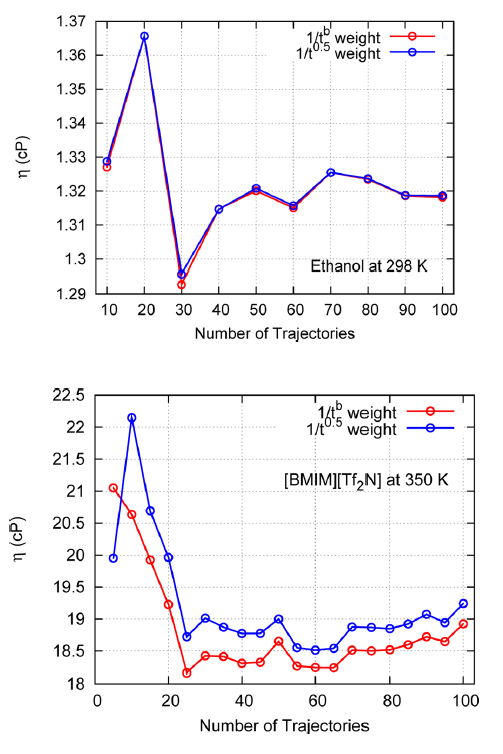
\includegraphics[width=3.2in]{ZhangFig7_12.png}
	\caption{Viscosity dependence on the exponent of the weighting model, $b$. $b = 0.52$ for Ethanol at 298K, top panel, while $b$ is between $0.60$ to $0.73$ for [BMIM][Tf$_2$N] at 350 K, bottom panel. Reprinted with permission from J. Chem. Theory Comput., 2015, 11 (8), pp 3537–3546. Copyright (2015) American Chemical Society. For further details, see Ref. \cite{Zhang2015}.}
	\label{fig:ZhangFig7_12}
\end{figure}

Ref. \cite{Zhang2015} also suggests that a cut-off time be implemented to improve the fit. They provide a heuristic that the cut-off time correspond to when the standard deviation is 40\% of the plateau value. Regardless of how the cut-off is determined, it is important to quantify the degree to which the estimated viscosity depends on this parameter. For example, Zhang et al. reported that the viscosity decreased by 0.8\% and 6.1\% when using a cut-off time corresponding to a standard deviation of 30\% or 20\% the plateau value, respectively. However, the magnitude of variability depends strongly on the system. We recommend that the author quantify the cut-off time dependence.

Furthermore, Ref. \cite{Zhang2015} recommends excluding short-time data from the fitting procedure. In Figure \ref{fig:ZhangFig4}, borrowed from Ref. \cite{Zhang2015}, we observe large oscillations at very short times, ca. $t < 2$ ps. A weighting function with a $t^{-b}$ form assigns an inappropriately large weight to these short-time data points. Therefore, it is important to exclude data in this short-time region from the model fitting. 

\begin{figure}[htb!]
	\centering
	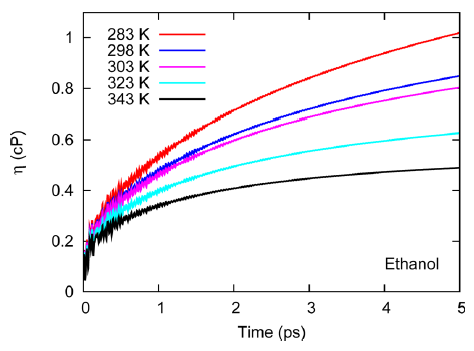
\includegraphics[width=3.2in]{ZhangFig4.png}
	\caption{Large fluctuations at very short time. Reprinted with permission from J. Chem. Theory Comput., 2015, 11 (8), pp 3537–3546. Copyright (2015) American Chemical Society. For further details, see Ref. \cite{Zhang2015}.}
	\label{fig:ZhangFig4}
\end{figure}  

%For example, plots of the estimated viscosity with respect to the weighting exponent and cut-off time, such as those shown in Figure \ref{fig:GK_tcut_b}, provide a quantitative measure of confidence in the viscosity value.

% compared two different values of $b$ in Figures 7, 12, and 13 (a fixed value of $b=2$ is used by \cite{ReyCastro2006})

%\begin{enumerate}
%	\item To smooth noise in Green-Kubo integral, we recommend performing independent replicate trajectories (i.e. different initial configurations or random seed to initialize velocities). The primary advantage of performing replicates as opposed to one longer simulation is the computational speed-up. Figure \ref{fig:PayalFig2}, taken from Payal et al. \cite{Payal2012}, demonstrates that an average of 10 replicate simulations of 2 ns length converges to the same value as a single 4 ns simulation. Since these replicates can be performed in parallel the computational time is reduced by a factor of two, in this example. However, Figure \ref{fig:ZhangFig8}, taken from \cite{Zhang2015}, demonstrates that if the length of each independent trajectory is too short the viscosity will not converge to the correct value, regardless of how many replicates are used.
%	%\item Averaging over multiple simulations with analytic fitting of integral provides a good way of smoothing noise and provides an objective means of determining the viscosity \cite{Zhang2015}.
%	% I think this point of averaging multiple simulations is important enough to merit its' own discussion
%	\item Replicates can provide a more rigorous uncertainty assessment. We recommend bootstrapping the uncertainties by randomly sampling which replicates are included in the average and data analysis procedure (see Green-Kubo for self-diffusivity).
%	\item The number of replicates used in literature varies widely. \cite{Payal2012} somewhat arbitrarily used 10 replicates whereas \cite{Zhang2015} performed a systematic investigation of the minimal number of replicates required for convergence. They observed that a value of 30-40 replicates was statistically equivalent to 100 replicates for their system. However, the necessary number of replicates depends on the system. Specifically, the compound, the temperature, the number of molecules, and the simulation time all influence the optimal number of replicates. Furthermore, because the uncertainty is inversely proportional to the square root of the number of replicates (see Figure 7 of \cite{Zhang2015} and Figure 8 of \cite{Ma2017}), increasing the number of replicates is a simple, fast, and direct way to reduce the uncertainty.
%	\item Report how the viscosity was estimated from the ``running integral''. There are three common methods:
%	\begin{enumerate}
%		\item A slightly ambiguous but common practice is to report an average that is obtained over a specified time interval. Due to large fluctuations at long times, the initial plateau at short times (around 10 ps) is typically the region of choice, see \cite{Fanourgakis2012,Chen2009}. However, it is important to explain how this time interval was selected (i.e. visual inspection, test of convergence, magnitude of fluctuations, etc.) and to quantify how much the estimated viscosity changes if time interval were modified.
%		\item An alternative method is to fit a model to the autocorrelation function before calculating the ``running integral.'' The integral of the model fit can then be evaluated in the limit as $t \to \infty$. This helps to overcome large fluctuations at long times and, thereby, reduces uncertainties. The primary difficulty is finding a model that can adequately match the autocorrelation function without introducing bias into the estimate of viscosity. A common function found in the literature is
%		\begin{equation} \label{eq:ACF_fit}
%		f(t)/f(0) = (1-C)cos(\omega t)\exp{(-t/\tau_f)^{\beta_f}} + C\exp{(-t/\tau_s)^{\beta_s}}
%		\end{equation}
%		where $C, \omega, \tau_f, \tau_s, \beta_f, \beta_s$ (and sometimes $f(0)$) are fitting parameters. $\omega$ is the frequency of rapid pressure oscillations, $\tau_f$ and $\beta_f$ are the time constant and exponent of fast relaxation in a stretched-exponential approximation, $\tau_s$ and $\beta_s$ are constants for slow relaxation, $C$ is the pre-factor that determines the weight between fast and slow relaxation, $f(t)$ is the autocorrelation function at time $t$, and $f(0)$ is the initial (time-zero) autocorrelation function \cite{GROMACS}. This method has been implemented successfully by \cite{Fanourgakis2012} where Figure \ref{fig:FanourgakisFig1}, from \cite{Fanourgakis2012}, demonstrates that Equation \ref{eq:ACF_fit} can reliably fit the autocorrelation function for this system. However, small deviations in the model fit can lead to significant bias in the estimated viscosity. Similar to the methods discussed previously, it is important to quantify the variability in viscosity that arises from the model fit. For example, we recommend bootstrapping the uncertainties of the model fit. Furthermore, if a weighting function or cut-off time is implemented the impact of these parameters should be discussed.
%		\item The method we recommend is to fit an analytic function directly to the ``running integral''. For example, \cite{ReyCastro2006} and \cite{Zhang2015} recommended fitting the ``running integral'' to a double-exponential function \begin{equation}
%		\eta(t) = A \alpha \tau_1 \left(1-\exp{(-t/\tau_1)}\right) + A (1-\alpha) \tau_2 \left(1-\exp{(-t/\tau_2)}\right)
%		\end{equation}
%		where $A, \alpha, \tau_1, $ and $\tau_2$ are fitting parameters. The primary advantage over the previous approach is that uncertainties in the model fit do not propagate through the integration. It is important to include a description of how the fit is performed, i.e. the objective function, weighting model, range of data included, etc. \cite{Zhang2015} recommend that the data be weighted by the inverse of the standard deviation with respect to time. They fit the standard deviation to a weighting model of the form $w \propto t^{-b}$, where $w$ is the weight, $t$ is the time, and $b$ is the weighting exponent. If such a model is utilized, we recommend that the author quantifies the uncertainty in the estimated viscosity due to the value of $b$, the weighting exponent. For example, \cite{Zhang2015} compared two different values of $b$ in Figures 7, 12, and 13 (a fixed value of $b=2$ is used by \cite{ReyCastro2006}). \cite{Zhang2015} also suggest that to improve the fit a cut-off time be implemented. They provide a heuristic that the cut-off time correspond to when the standard deviation is 40\% the plateau value. Regardless of how the cut-off is determined, it is important to quantify the degree to which the estimated viscosity depends on this parameter. For example, Zhang et al. reported that the viscosity decreased by 0.8\% and 6.1\% when using a cut-off time corresponding to a standard deviation of 30\% or 20\% the plateau value, respectively. However, the magnitude of variability depends strongly on the system. We recommend that the author demonstrate the cut-off time dependence. For example, plots of the estimated viscosity with respect to the weighting exponent and cut-off time, such as those shown in Figure \ref{fig:GK_tcut_b}, provide a quantitative measure of confidence in the viscosity value.
%	\end{enumerate}
%RAM: Again, I think we want to avoid any discussion of force field accuracy
%	\item Force fields: systematic consideration of the intra- vs. inter- molecular potential models; UA, vs. AUA vs. EA differences may be significant. For charged systems, polarizable force fields might be needed to get accurate results. Some studies have suggested that united-atom models are not capable of accurately reproducing viscosity and, therefore, anisotropic-united-atom or all-atom models are needed \cite{Allen1987,Payal2012,Mondello1997}. However, other studies have shown that with the appropriate tuning of the united-atom force field parameters viscosity can be accurately predicted without significant deprecation of other properties \cite{Gordon2006}. \cite{Ungerer2007} discusses different test cases (i.e. state points, compound structures) where united-atom or anisotropic-united-atom models are adequate and inadequate for predicting viscosity.
%
%
%\end{enumerate}
%
%\begin{figure}[htb!]
%	\centering
%	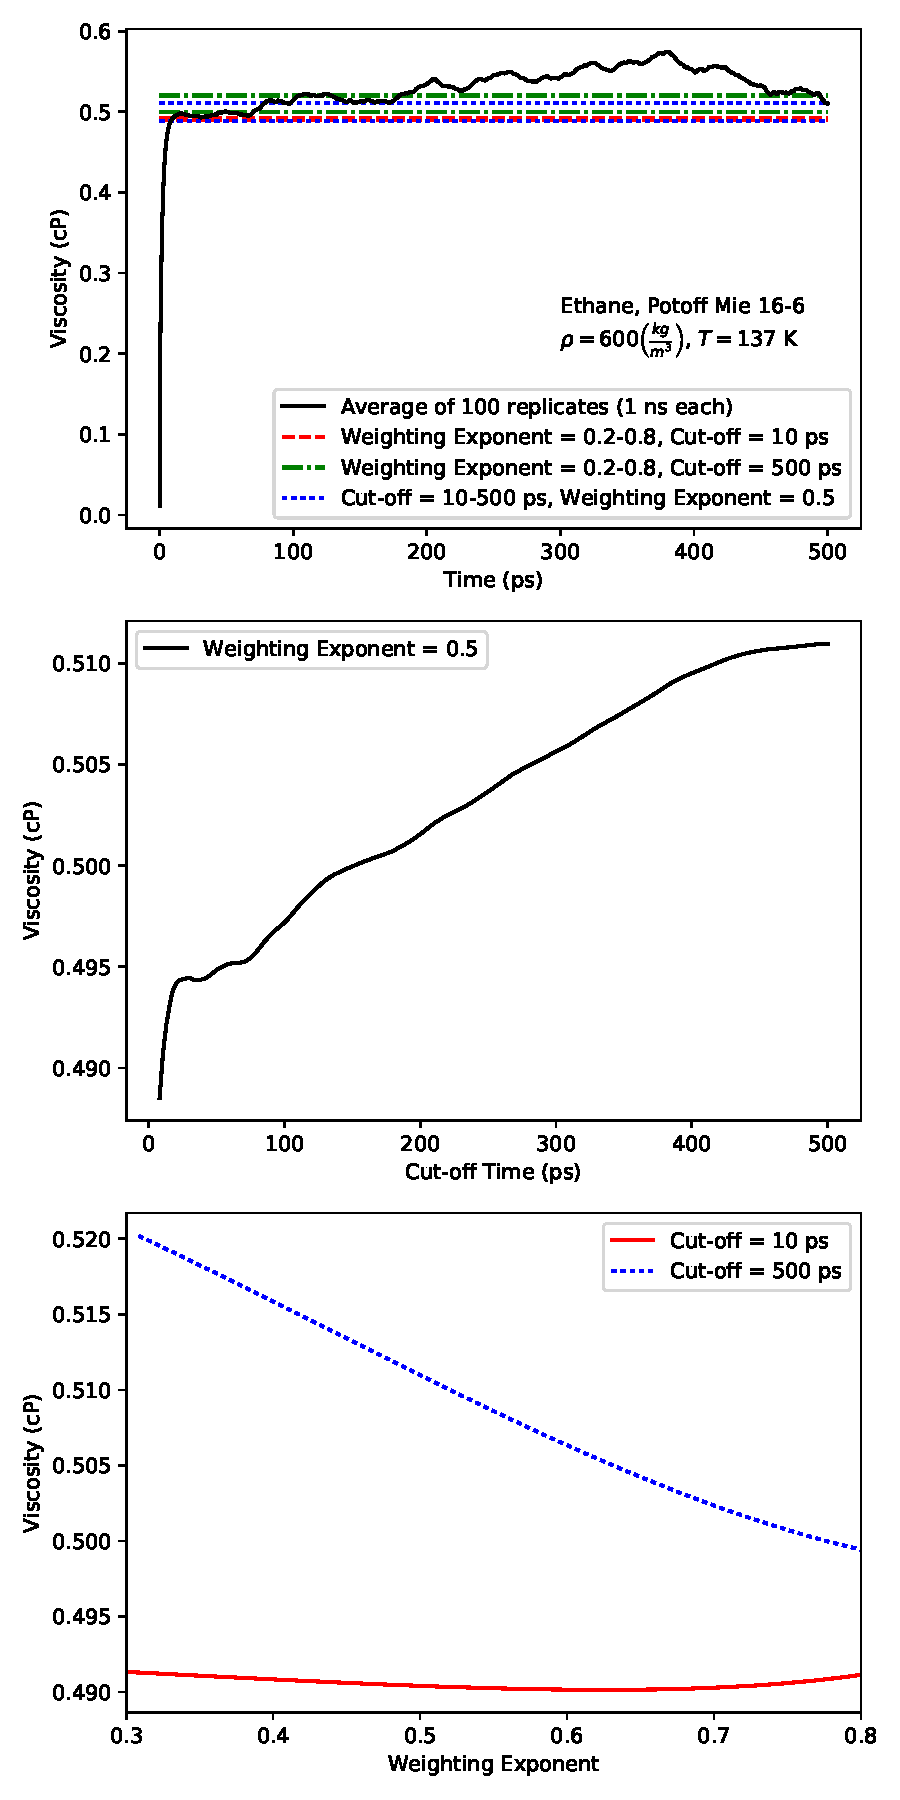
\includegraphics[width=3.2in]{GreenKubo_tcut_b_dependence.pdf}
%	\caption{Uncertainty quantification of cut-off time and weighting exponent for method proposed by Zhang et al. Results are shown for a system of 400 united-atom ethane molecules, simulated with the \cite{Potoff2009} model at saturated liquid density for a temperature of 137 K. Top panel plots the Green-Kubo running integral as average of 100 replicates, each of 1 ns duration. The dashed lines represent different estimates of uncertainty attributed to the cut-off time or the weighting exponent. Middle panel plots the estimated viscosity as a function of cut-off time for a fixed weighting exponent. Bottom panel plots the estimated viscosity as a function of the weighting exponent for two different cut-off times. For longer cut-off times, the viscosity depends strongly on the weighting exponent (around $\pm 2$\%) while shorter times are much less dependent (around $\pm 0.1$\%). For the recommended weighting exponent, the cut-off time can cause the viscosity to vary by around $\pm 2$\%. Note that these results may depend strongly on the state point and number of molecules.}
%	\label{fig:GK_tcut_b}
%\end{figure}

\subsection{Viscosity: Einstein} \label{sec:Viscosity Einstein}

%\subsubsection{Improved precision} \label{sec:Viscosity:Einstein: Improved precision}
%
%%Similar to the Green-Kubo approach for viscosity, the key to obtaining precise estimates with the Einstein approach is to average multiple replicate simulations.
%
%The viscosity with respect to time is estimated from the slope of the Einstein integral. Thus, the average of replicates can be performed in one of two ways. The first option is to calculate the viscosity (i.e. the slope) with respect to time for each replicate and then average the replicate viscosities. However, this approach results in large fluctuations and, therefore, large uncertainties. The second, and recommended, method is to average the Einstein integral of the multiple replicates. The resulting Einstein integral is often linear over a large time interval if sufficient replicates are used. Subsequently, the slope is determined from this average Einstein integral. Fortunately, with sufficient replicate simulations the slope tends to be fairly constant over intermediate and long-time intervals. The number of replicates needed has not been rigorously investigated as it has for the Green-Kubo approach. For this reason, we recommend creating a plot of viscosity with respect to number of replicates (see Figure \ref{fig:ZhangFig8}) to determine when sufficient replicates have been simulated. It is our experience that the necessary number of replicates is similar to that for Green-Kubo. As recommended for Green-Kubo, we also recommend bootstrapping the uncertainty. This is done by randomly sampling which replicates are included in the average Einstein integral, calculating the viscosity from the slope, and producing a distribution of these viscosity values from thousands of different random sets of replicates.

\subsubsection{Data analysis} \label{sec:Viscosity:Einstein: Data analysis}

%Similar to the Einstein approach for self-diffusivity, in general, the initial time should be discarded. Since the Einstein relation is valid in the limit of infinite time, it is common to fit the slope at long time. However, it is also common to fit the slope to an intermediate time interval. We recommend that the author explain why the slope was calculated using a given time interval and how much variability is introduced if a different region is selected. For example, similar to the bootstrap method discussed in Sec.\ \ref{sec:General: Uncertainty}, a useful measure of uncertainty would be the range of $\eta$ values obtained by analyzing numerous (order of 100) different time regions.

Since the Einstein relation is valid in the limit of infinite time, in theory the slope should only be computed at long time. Unfortunately, by contrast with self-diffusivity, the long-time trend from a single run is often non-linear (recall Figure \ref{fig:Einstein_3terms_30replicates}). Replicate simulations are typically necessary to obtain a well-behaved long-time trend. For example, Figure \ref{fig:Einstein_3terms_30replicates} demonstrates that the replicate-averaged Einstein integral is approximately linear over a large time interval (using 30 replicate simulations). Therefore, if sufficient replicates are used it is possible to compute a reliable slope (viscosity) at the long-time limit.

However, as observed in the inset of Figure \ref{fig:Einstein_3terms_30replicates}, the Einstein integral becomes nearly linear for a single simulation after a few ps. For these reasons, it is common to fit the slope from a single simulation over an intermediate time interval, e.g. 5 to 50 ps. We only recommend calculating the slope from an intermediate time interval if performing a large number of replicate simulations is too computationally expensive. Also, as mentioned in Sec. \ref{sec:Viscosity}, the Einstein approach is likely preferred over the Green-Kubo approach only in this scenario. With a single simulation (or a small number of replicate simulations), we recommend that the author explain why the slope was calculated using a given intermediate time interval and how much variability is introduced if a different region is selected. 

For example, Figure \ref{fig:Einstein_slope_time_interval} helps visualize the uncertainty in $\eta$ due to the time interval used to compute the slope. Panels a) and b) are obtained from the respective single and 30 replicate simulation results presented previously in Figure \ref{fig:Einstein_3terms_30replicates}. Panel a) demonstrates that determining $\eta$ from a single run depends strongly on the time interval, while Panel b) shows that $\eta$ is much less dependent on the time interval when obtained from 30 replicate simulations.

\begin{figure}[htb!]
	\centering
	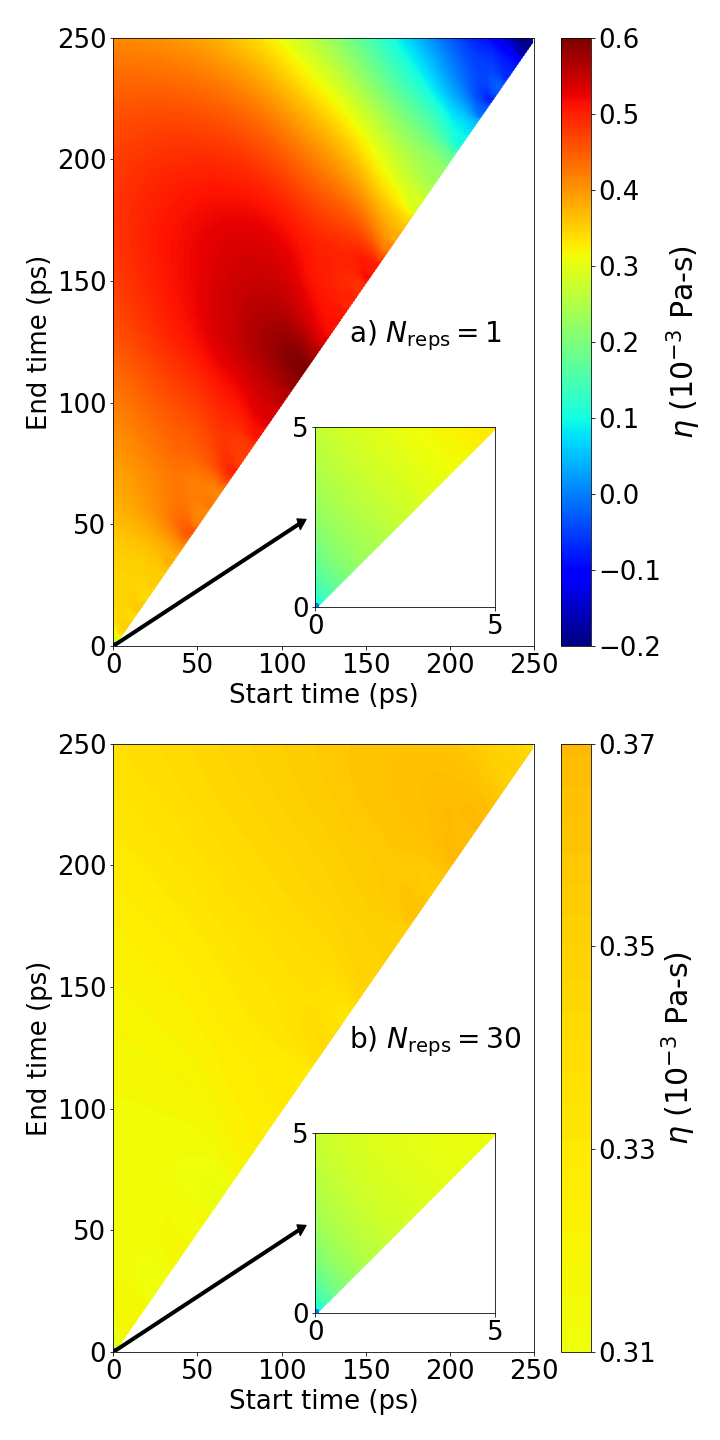
\includegraphics[width=3.2in]{Einstein_slope_time_interval.png}
	\caption{Dependence of $\eta$ on the time interval used to compute the Einstein slope. For example, ``start time'' $=$ 50 ps and ``end time'' $=$ 200 ps computes the slope from $t = 50$ to $200$ ps of $\displaystyle \frac{V}{2 k_B T N_{\rm reps}} \sum_{n=1}^{N_{\rm reps}} \left\langle \int_0^t \tau_{\alpha\beta,n}(t') dt' \right\rangle_{t_0}$. Panels a) and b) correspond to a single simulation and 30 replicate simulations, respectively. The same color scale is used in both panels, but Panel b) also includes a zoomed-in color bar. Simulation data are the same as those presented in Figure \ref{fig:Einstein_3terms_30replicates}.}
	\label{fig:Einstein_slope_time_interval}
\end{figure}

% similar to the bootstrap method discussed in Sec.\ \ref{sec:General: Uncertainty}, a useful measure of uncertainty is the range of $\eta$ values obtained by analyzing numerous (order of 100) different time regions.

%Regardless of whether the viscosity is determined from a single run at intermediate times or multiple runs at long times

%The recommended method to avoid arbitrarily selecting an intermediate time interval is to average the Einstein integral for multiple replicate simulations, i.e. $\displaystyle \frac{1}{N_{\rm reps}} \sum_{n=1}^{N_{\rm reps}} \left\langle \left(\int_{0}^{t}dt' \tau_{n}(t')\right)^2 \right\rangle_{t_0}$ where $N_{\rm reps}$ is the number of replicates. For example, Figure \ref{fig:Einstein_3terms_30replicates} demonstrates that the replicate-averaged Einstein integral is approximately linear over a large time interval (using 30 replicate simulations). Therefore, if sufficient replicates are used it is possible to compute a reliable slope (viscosity) at the long-time limit.

%The recommended method to avoid arbitrarily selecting an intermediate time interval is to average the Einstein integral for multiple replicate simulations
%\begin{equation}
%\eta = \displaystyle \frac{V}{20 k_B T N_{\rm reps}} \lim_{t\to\infty} \frac{d}{dt} \sum_{n=1}^{N_{\rm reps}} \sum_i \sum_j \left\langle \int_0^t \tau_{ij,n}^{os}(t') dt' \right\rangle_{t_0}
%\label{eq:Einwonder_replicates}
%\end{equation}
%where $N_{\rm reps}$ is the number of replicates. For example, Figure \ref{fig:Einstein_3terms_30replicates} demonstrates that the replicate-averaged Einstein integral is approximately linear over a large time interval (using 30 replicate simulations). Therefore, if sufficient replicates are used it is possible to compute a reliable slope (viscosity) at the long-time limit.


%Since the viscosity is estimated from the slope of the Einstein integral, the average of replicates can be performed in one of two ways. The first option is to calculate the viscosity (i.e. the slope) with respect to time for each replicate and then average the replicate viscosities. However, as demonstrated previously in Figure \ref{fig:Einstein_3terms_30replicates}, the long-time slope from a single run can result in extremely erroneous estimates of viscosity.
%
%The second, and recommended, method when implementing the Einstein approach is to average $\displaystyle \left\langle \left(\int_{0}^{t}dt' \tau_{\alpha,\beta}(t')\right)^2 \right\rangle_{t_0}$ (referred to as the Einstein integral) for multiple replicates. The replicate-averaged Einstein integral is often linear over a large time interval if sufficient replicates are used (see Figure \ref{fig:Einstein_3terms_30replicates}). Therefore, a reliable slope (viscosity) can be computed at the long-time limit, rather than arbitrarily computing the slope at shorter times.

%Subsequently, the slope is determined from this average Einstein integral. 

%Fortunately, with sufficient replicate simulations the slope tends to be fairly constant over intermediate and long-time intervals. 

Since the slope for an intermediate time interval is less theoretically rigorous and depends strongly on user judgment, the recommended method, when computationally feasible, is to average the Einstein integral for multiple replicate simulations, i.e. Equation \ref{eq:Einwonder_replicates}. The number of replicates needed has not been rigorously investigated as it has for the Green-Kubo approach. For this reason, we recommend creating a plot of viscosity with respect to number of replicates (see Figure \ref{fig:ZhangFig8}) to determine when sufficient replicates have been simulated. It is our experience that the necessary number of replicates is similar to that for Green-Kubo. 

Similar to the Green-Kubo recommendation, we also recommend bootstrapping the uncertainty for the Einstein approach (see Sec.\ \ref{sec:General: Uncertainty}). This is done by randomly sampling which replicates are included in the replicate-averaged Einstein integral, calculating the viscosity from the slope, and producing a distribution of these viscosity values from hundreds or thousands of different random replicate sets. 

In addition, we recommend bootstrapping the time interval uncertainty, i.e. computing the slope for hundred or thousands of different time intervals. This approach is especially important if analyzing intermediate time intervals from a single simulation. For example, from Figure \ref{fig:Einstein_slope_time_interval} Panel a) we would report the distribution of $\eta$ values obtained from randomly selected time intervals with a ``start time'' greater than 5 ps and an ``end time'' less than 50 ps. 

%For example, for the single and 30 replicate simulations in Figure \ref{fig:Einstein_slope_time_interval} Panels a) and b), respectively, we can report the variability  a useful measure of uncertainty is the range of $\eta$ values obtained by analyzing numerous (order of 100) different time regions.

\subsection{Viscosity: Special topics} \label{sec:Viscosity Special topics}

The GROMACS manual reports that viscosity ``is very dependent on the treatment of the electrostatics. Using a (short) cut-off results in large noise on the off-diagonal pressure elements, which can increase the calculated viscosity by an order of magnitude.'' \cite{GROMACS,Hess2002} Therefore, when computing viscosities for systems with electrostatics, it is extremely important to investigate the effect of cut-off distance. This can be done by performing simulations with variable Coulombic cut-off lengths, typically 0.9, 1.2, and 1.4 nm. We also recommend investigating whether the estimated viscosity depends strongly on the algorithm for computing the electrostatics, i.e. particle mesh Ewald, etc. \cite{GROMACS} 

Similarly, we suspect that the viscosity also depends on the van der Waals cut-off length and/or if a cut-and-shift, force-switch, or truncated (with or without tail corrections) potential is implemented \cite{GROMACS}. For these reasons, we strongly recommend reporting how the non-bonded (electrostatics and van der Waals) interactions are computed. 

\section{Conclusions} \label{Conclusions}
%RAM: I have commented out DJC original conclusion section, and copied a slightly modified version
%Molecular simulation is commonly used to predict transport properties, however, without careful simulation design and acute analysis, results may not be meaningful. For example, an EMD simulation with an insufficient number of molecules can severely underestimate self-diffusivity. This work outlines the best practices in the design and analysis of MD simulations for transport properties.
%
%For self-diffusivity, it is suggested that the Einstein method is employed. In liquid systems, the NVE ensemble is suggested over the NVT ensemble due to the potential interference of the thermostats in self-diffusivity prediction. Uncertainty is reduced by running multiple independent simulations, allowing for a more thorough sampling of the system's possible states. Multiple runs at different system sizes can be used to extrapolate the infinite system size limit prediction for self-diffusivity. Atom positions are recommended to be outputted 1000 times over a production run, however, the user can choose to output less frequently to reduce file size or more frequently for potentially increased accuracy. To ensure simulations are run long enough for the dynamics of the system to be fully emulated, the user can run a series of simulations at differing lengths, and observe deviation in estimated self-diffusivity with changes in simulation time. The system's degree of exploration of configuration space can be estimated by calculating the MSD of the molecules and comparing it to the radius of gyration and box length. The MSD should be greater than the radius of gyration, and ideally, on the order of the box length. In post-simulation analysis, best practice improves precision by averaging the velocity autocorrelation function over all molecules and over multiple time origins. Some judgment by the user is necessary to decide where the slope is measured for the Einstein approach, and it is important that the user communicate the approach used and justify how the decision was made. Measures should be taken to rigorously estimate the precision of the self-diffusivity prediction, a method of bootstrapping these uncertainties is detailed in this work.
%
%For viscosity, the Green-Kubo approach is recommended, although the Einstein method may be preferred with certain systems. It is worth noting that NEMD simulations are highly preferred for moderate to high viscosity materials (more than 20 cP or so). The NVE ensemble is suggested, but some success has been found using the NVT ensemble \cite{Shirts2013,Fanourgakis2012}. Because it is a collective property, viscosity requires significantly more data than self-diffusivity. The simulation length of each trajectory should typically be at least an order of magnitude greater than the Green-Kubo integral plateau time. This can be more precisely determined by comparing the Green-Kubo integrals of varying simulation lengths. Due to their slower dynamics, more viscous materials require longer simulation times. Stress tensor components are recommended to be outputted every 5 to 10 fs. System size seems to be of little impact on viscosity prediction (see Figures \ref{fig:MoultosFig3}-\ref{fig:ZhangFig9}), however, it is still recommended that the user justify their choice of system size by plotting $N^{-1/3}$ versus predicted viscosity. Any trend observed would suggest system size effects, and an infinite system size result could be estimated from a linear fit. In post-simulation data processing, it is recommended to average over all six independent components of the stress tensor to enhance precision. The number of replicates a system needs can vary greatly depending on the compound, number of molecules, temperature, and simulation length. Replicates required can be investigated by plotting variance in viscosity versus number of replicates (on the order of 10 to 30), wherein a trend may indicate that more replicates are needed. It is recommended that the viscosity is estimated from the Green-Kubo equation by fitting the running integral to a double-exponential function as specified by Zhang et al. \cite{Zhang2015} (see Section \ref{sec:Viscosity:Green-Kubo: Data analysis}).
%
%The focus of the current work is outlining best practices in EMD for self-diffusivity and viscosity prediction. This work may be expanded on in the future with NEMD techniques or best practices for other transport properties.

Molecular simulation is commonly used to predict transport properties. However, without careful simulation design and acute analysis, results may not be meaningful. This work outlines the best practices in the design and analysis of equilibrium molecular dynamics simulations for self-diffusivity and viscosity prediction. We anticipate future studies discussing best practices for non-equilibrium molecular dynamics techniques or additional transport properties.

For self-diffusivity, we recommend employing the Einstein method. In liquid systems, the $NVE$ ensemble is suggested over the $NVT$ ensemble due to the potential interference of the thermostats in self-diffusivity prediction. Uncertainty is reduced by running multiple independent simulations, allowing the system to more thoroughly sample the possible states. We recommend multiple runs at different system sizes to extrapolate the infinite system size limit prediction for self-diffusivity. Atom positions are recommended to be outputted 1000 times over a production run, however, the user can choose to output less frequently to reduce file size or more frequently for potentially increased accuracy. To ensure simulations are run long enough for the dynamics of the system to be fully emulated, the user can run a series of simulations at differing lengths, and observe deviation in estimated self-diffusivity with changes in simulation time. The degree of configuration space exploration can be estimated by calculating the mean squared displacements of the molecules and comparing to the radius of gyration and box length. The root MSD should be greater than the radius of gyration, and ideally, on the order of the box length. In post-simulation analysis, best practice improves precision by averaging the velocity autocorrelation function over all molecules and over multiple time origins. Some judgment by the user is necessary to decide where the slope is measured for the Einstein approach, and it is important that the user communicate the approach used and justify how the decision was made. Measures should be taken to rigorously estimate the precision of the self-diffusivity prediction, where we recommend bootstrapping the uncertainties.

For viscosity, the Green-Kubo approach is recommended, although the Einstein method may be preferred with certain systems, i.e. if replicate simulations are too computationally expensive. It is worth noting that NEMD simulations are highly preferred for moderate to high viscosity materials (more than 20 to 50 cP). The $NVE$ ensemble is suggested, but some success has been found using the $NVT$ ensemble \cite{Shirts2013,Fanourgakis2012}. As a collective property, viscosity requires significantly more data than self-diffusivity. The simulation length of each trajectory should typically be at least an order of magnitude greater than the Green-Kubo integral plateau time. This can be more precisely determined by comparing the Green-Kubo integrals of varying simulation lengths. Due to their slower dynamics, more viscous materials require longer simulation times. Stress tensor components are recommended to be outputted every 5 to 10 fs. System size seems to be of little impact on viscosity prediction (see Figures \ref{fig:MoultosFig3}-\ref{fig:ZhangFig9}), however, it is still recommended that the user justify their choice of system size by plotting $N^{-1/3}$ versus predicted viscosity. Any trend observed would suggest system size effects, and an infinite system size result could be estimated from a linear fit. In post-simulation data processing, it is recommended to average over all six independent components of the stress tensor to enhance precision. The number of replicates a system needs can vary greatly depending on the compound, number of molecules, temperature, and simulation length. It is recommended that the viscosity is estimated from the Green-Kubo equation by fitting the running integral to a double-exponential function as specified by Zhang et al. \cite{Zhang2015} (see Section \ref{sec:Viscosity:Green-Kubo: Data analysis}).

\section*{Acknowledgments}

This research was performed while R.A.M. held a National Research Council (NRC) Postdoctoral Research Associateship at the National Institute of Standards and Technology (NIST). D.M.Z. acknowledges support from NIH Grant GM115805.

\section*{Disclaimer}

Certain commercially available items may be identified in this paper. This identification does not imply recommendation by NIST, nor that it is the best available for the purposes described.

%\nocite{*} % This command displays all refs in the bib file
\bibliography{transport_properties}

%%%%%%%%%%%%%%%%%%%%%%%%%%%%%%%%%%%%%%%%%%%%%%%%%%%%%%%%%%%%
%%% APPENDICES
%%%%%%%%%%%%%%%%%%%%%%%%%%%%%%%%%%%%%%%%%%%%%%%%%%%%%%%%%%%%

\end{document}
